\documentclass[11pt,letterpaper]{article}

\usepackage[margin=1in]{geometry}
\usepackage{amsmath,amssymb}
\usepackage{graphicx}
\usepackage{booktabs}
\usepackage{caption}
\usepackage{subcaption}
\usepackage{float}
\usepackage{multirow}
\usepackage{array}
\usepackage{enumitem}
\usepackage{hyperref}
\usepackage{setspace}

\hypersetup{colorlinks=true, linkcolor=blue, citecolor=blue, urlcolor=blue}
\graphicspath{{results/}}

% ============================================================
\begin{document}

% -----------------------------------------------------------
% 1. Title Page
% -----------------------------------------------------------
\begin{titlepage}
  \centering
  \vspace*{2cm}
  {\LARGE\bfseries Assignment \#2: Novel DCNN Architecture,\\[0.4em]
   Transfer Learning, and Ensemble Methods}\\[1.2cm]
  {\large COMP/EECE 7/8740 --- Neural Networks}\\[0.4cm]
  {\large Spring 2026}\\[2.5cm]
  \begin{tabular}{rl}
    \textbf{Student Name:}   & \textit{Jace King}\\[0.5cm]
    \textbf{Student ID:}     & \textit{U00969076}\\[0.5cm]
    \textbf{Submission Date:}& March 2026\\
  \end{tabular}
  \vfill
\end{titlepage}

% -----------------------------------------------------------
% 2. Abstract  (starts on second page)
% -----------------------------------------------------------
\begin{abstract}
This report presents \textbf{CompactNet}, a novel deep convolutional neural network
built on residual bottleneck blocks, and evaluates it for image classification on
Tiny ImageNet-200 (200 classes) and CIFAR-100 (100 classes).
Three activation functions are compared:
ReLU, GELU, and the custom \emph{Rational Swish} (RSwish) developed in Assignment~1.
All variants are optimised with AdamW and a cosine-annealing learning-rate schedule.
On Tiny ImageNet-200, RSwish achieves the best test accuracy of \textbf{47.83\%},
outperforming ReLU (42.87\%) and GELU (45.10\%).
Transfer learning from Tiny ImageNet to CIFAR-100 lifts accuracy from
44.63\% (scratch) to \textbf{63.35\%}, and a soft-voting ensemble of three
independently fine-tuned RSwish models further improves performance to
\textbf{64.65\%}.
Under an industrial confidence threshold of 0.9, the ensemble attains
\textbf{96.32\%} accuracy with 28.0\% coverage, demonstrating the practical
utility of ensemble-based uncertainty estimation.
\end{abstract}

\newpage
\tableofcontents
\newpage

% -----------------------------------------------------------
% 3. Introduction
% -----------------------------------------------------------
\section{Introduction}

\subsection{Problem Definition}

Image classification is a foundational computer-vision task in which a model
assigns a semantic label to an input image from a fixed category set.
This assignment addresses two benchmarks:
\begin{itemize}[noitemsep]
  \item \textbf{Tiny ImageNet-200}: 200 classes, $64\!\times\!64$ colour images,
        down-sampled to $32\!\times\!32$ in our pipeline.
  \item \textbf{CIFAR-100}: 100 classes, native $32\!\times\!32$ colour images.
\end{itemize}
Beyond raw accuracy, the assignment requires demonstrating the incremental value of
transfer learning and ensemble methods, and evaluating model reliability via
high-confidence selective prediction.

\subsection{Background and Related Work}

Deep convolutional neural networks have dominated visual recognition since
AlexNet~\cite{krizhevsky2012imagenet}.
Key advances informing this work include:

\begin{itemize}[noitemsep]
  \item \textbf{Residual Networks (ResNet)}~\cite{he2016deep}: skip connections allow
        gradients to flow unimpeded through very deep networks.
  \item \textbf{Densely Connected Networks (DenseNet)}~\cite{huang2017densely}: each
        layer receives concatenated feature maps from all preceding layers, promoting
        feature reuse.
  \item \textbf{Bottleneck blocks}: introduced in ResNet-50/101, a
        $1\!\times\!1\!\to\!3\!\times\!3\!\to\!1\!\times\!1$ convolution sequence
        reduces parameter count while increasing representational depth.
  \item \textbf{Batch Normalisation (BN)}~\cite{ioffe2015batch}: normalises activations
        per mini-batch, accelerating training and acting as a regulariser.
  \item \textbf{Global Average Pooling (GAP)}~\cite{lin2013network}: replaces
        large fully-connected layers, reducing parameters and providing spatial
        invariance.
  \item \textbf{Transfer Learning}: pre-training on a large source dataset and
        fine-tuning on a smaller target task is a powerful strategy for limited data.
  \item \textbf{Ensemble Methods}~\cite{opitz1999popular}: combining predictions from
        multiple independently trained models reduces variance and improves
        generalisation.
\end{itemize}

\subsection{Objectives and Contributions}

The primary objectives are:
\begin{enumerate}[noitemsep]
  \item Design and train a novel DCNN (CompactNet) on Tiny ImageNet-200, comparing
        three activation functions: ReLU, GELU, and the custom RSwish from
        Assignment~1.
  \item Evaluate transfer learning by fine-tuning the best-performing model on
        CIFAR-100 and comparing it against a from-scratch baseline.
  \item Build a soft-voting ensemble of three independently trained models and
        quantify its benefit over a single model.
  \item Report accuracy, precision, recall, F1-score, ROC-AUC, and PR-AUC for all
        settings at both full coverage and a high-confidence threshold of 0.9.
\end{enumerate}

% -----------------------------------------------------------
% 4. Methodology
% -----------------------------------------------------------
\section{Methodology}

\subsection{Overall Pipeline}

\begin{enumerate}[noitemsep]
  \item \textbf{Task 1a --- Activation comparison}: Train CompactNet with ReLU,
        GELU, and RSwish on Tiny ImageNet-200 for 100 epochs; select the best
        activation by test accuracy.
  \item \textbf{Task 1b --- Transfer learning}: Using the winning activation (RSwish),
        train CompactNet on CIFAR-100 (i) from scratch with He initialisation and
        (ii) fine-tuned from the Tiny ImageNet checkpoint.
  \item \textbf{Task 2 --- Ensemble}: Train three RSwish CompactNet instances on
        CIFAR-100, each initialised from the Tiny ImageNet checkpoint but with
        independent random seeds (42, 43, 44); combine predictions via soft voting.
  \item Evaluate all models on held-out test sets.
\end{enumerate}

\subsection{Data Preprocessing}

\paragraph{Tiny ImageNet-200.}
Images are originally $64\!\times\!64$ and are resized to $32\!\times\!32$ to match
the CIFAR-100 input size and enable weight transfer.
The official 100k-image training split is divided 80/20 per class (fixed seed~$=0$)
into training and validation subsets.
The official 10k-image validation split is used as the held-out test set.
Channel-wise normalisation uses dataset statistics:
$\mu = (0.4802, 0.4481, 0.3975)$,
$\sigma = (0.2770, 0.2691, 0.2821)$.
Training augmentations are \texttt{RandomCrop(32, padding=4)} and
\texttt{RandomHorizontalFlip}.

\paragraph{CIFAR-100.}
Native $32\!\times\!32$ images are normalised with
$\mu = (0.5071, 0.4867, 0.4408)$,
$\sigma = (0.2675, 0.2565, 0.2761)$.
The 50k-image training split is divided 80/20 per class (seed~$=0$);
the 10k-image test split is the held-out test set.
The same augmentations as Tiny ImageNet are applied at training time.

\subsection{Evaluation Strategy}

All models are assessed at two operating points:
\begin{itemize}[noitemsep]
  \item \textbf{Full coverage}: every test sample is classified.
  \item \textbf{High-confidence (conf~$\geq 0.9$)}: only samples whose maximum
        softmax probability exceeds 0.9 are scored;
        \emph{coverage} (fraction of retained samples) is always reported.
\end{itemize}

% -----------------------------------------------------------
% 5. Neural Network Architecture
% -----------------------------------------------------------
\section{Neural Network Model Descriptions}

\subsection{CompactNet Design Rationale}

CompactNet is a compact residual network designed for $32\!\times\!32$ input images.
Inspired by ResNet's bottleneck blocks~\cite{he2016deep} and the channel-compression
principle of $1\!\times\!1$ convolutions~\cite{lin2013network}, it achieves a
favourable accuracy-to-parameter ratio with exactly
$\mathbf{1{,}051{,}272}$ trainable parameters for the 200-class head
($999{,}972$ for the 100-class CIFAR-100 head).

\subsubsection{Bottleneck Residual Block}

Each residual block applies a three-layer bottleneck:
\begin{equation}
  \mathbf{y} = \sigma\!\Bigl(
    \mathbf{x}' +
    \mathrm{BN}\!\bigl(
      \mathbf{W}_3 \cdot
      \sigma\!\bigl(
        \mathrm{BN}\!\bigl(
          \mathbf{W}_2 * \sigma\!\bigl(
            \mathrm{BN}(\mathbf{W}_1 \cdot \mathbf{x})
          \bigr)
        \bigr)
      \bigr)
    \bigr)
  \Bigr),
  \label{eq:bottleneck}
\end{equation}
where $\mathbf{W}_1$ is a $1\!\times\!1$ convolution that compresses channels by
$4\times$ (bottleneck width $= C_\text{out}/4$), $\mathbf{W}_2$ is a $3\!\times\!3$
convolution on the compressed representation, $\mathbf{W}_3$ is a $1\!\times\!1$
convolution that expands channels back, $\sigma$ is the chosen activation, and
$\mathbf{x}'$ is the identity or a $1\!\times\!1$ projection shortcut whenever spatial
resolution or channel count changes.
Compressing to $C_\text{out}/4$ channels before the $3\!\times\!3$ reduces the
parameter count of that layer by $16\times$ relative to a plain
$3\!\times\!3$ layer of the same output width.

\subsubsection{Full Architecture}

Table~\ref{tab:arch} summarises CompactNet.
At every transition, the first block in a stage uses stride 2 to halve spatial
resolution while doubling the channel count; subsequent blocks maintain dimensions.

\begin{table}[H]
  \centering
  \caption{CompactNet layer-wise summary ($32\!\times\!32\!\times\!3$ input,
           200-class output).}
  \label{tab:arch}
  \begin{tabular}{llccc}
    \toprule
    \textbf{Stage} & \textbf{Block type} &
    \textbf{Out channels} & \textbf{Strides} & \textbf{Output size} \\
    \midrule
    Stem    & Conv $3\!\times\!3$, BN, Act & 64  & 1      & $32\!\times\!32\!\times\!64$  \\
    Stage 1 & Bottleneck $\times 2$        & 64  & 1,1    & $32\!\times\!32\!\times\!64$  \\
    Stage 2 & Bottleneck $\times 2$        & 128 & 2,1    & $16\!\times\!16\!\times\!128$ \\
    Stage 3 & Bottleneck $\times 3$        & 256 & 2,1,1  & $8\!\times\!8\!\times\!256$   \\
    Stage 4 & Bottleneck $\times 2$        & 512 & 2,1    & $4\!\times\!4\!\times\!512$   \\
    GAP     & AdaptiveAvgPool2d            & 512 & ---    & $1\!\times\!1\!\times\!512$   \\
    Dropout & $p = 0.5$                    & 512 & ---    & 512                           \\
    Head    & Linear                       & 200 & ---    & 200                           \\
    \bottomrule
  \end{tabular}
\end{table}

\subsection{Activation Functions}

\paragraph{ReLU.}
$\mathrm{ReLU}(x) = \max(0,\,x)$.
Piecewise-linear and computationally efficient, but unresponsive (zero gradient)
for negative inputs, which can cause dying-neuron pathologies in deep networks.

\paragraph{GELU.}
$\mathrm{GELU}(x) = x\,\Phi(x)$, where $\Phi$ is the standard-normal
CDF~\cite{hendrycks2016gelu}.
A smooth, stochastically-motivated non-linearity widely used in transformer models.

\paragraph{RSwish (custom, Assignment~1).}
The Rational Swish replaces the exponential sigmoid in Swish with an algebraic
softsign approximation, eliminating transcendental operations entirely:
\begin{equation}
  \mathrm{RSwish}(x)
  = x \cdot \frac{1 + \dfrac{x}{1+|x|}}{2}.
  \label{eq:rswish}
\end{equation}
The rational factor $r(x) = \bigl(1 + x/(1+|x|)\bigr)/2$ maps
$(-\infty,+\infty)\!\to\!(0,1)$, matching the true sigmoid's range without any
exponentials.
The result is a smooth, non-monotone activation that gates the pre-activation
value—analogous to Swish—at a fraction of the computational cost.

\subsection{Optimisation and Regularisation}

\begin{itemize}[noitemsep]
  \item \textbf{Optimiser}: AdamW~\cite{loshchilov2019adamw} with decoupled
        weight decay $\lambda = 10^{-4}$.
  \item \textbf{LR schedule}: Cosine annealing,
        $\eta_{\min} = 10^{-2}\,\eta_0$.
  \item \textbf{Task~1 (Tiny ImageNet)}: $\eta_0 = 10^{-3}$, 100 epochs, batch 64.
  \item \textbf{Task~1/2 (CIFAR-100)}: $\eta_0 = 10^{-4}$, 50 epochs, batch 64.
  \item \textbf{Weight initialisation}: He (Kaiming) initialisation~\cite{he2015delving}
        for all Conv2d and Linear layers.
  \item \textbf{Dropout}~\cite{srivastava2014dropout}: $p = 0.5$ applied before the classification head.
  \item \textbf{Loss function}: Cross-entropy.
\end{itemize}

For the CIFAR-100 fine-tuning and ensemble experiments the 200-class classification
head is replaced with a freshly He-initialised 100-class Linear layer, while all
convolutional weights are loaded from the Tiny ImageNet checkpoint.

% -----------------------------------------------------------
% 6. Experiments and Results
% -----------------------------------------------------------
\section{Experiments and Results}

\subsection{Dataset Description}

\paragraph{Tiny ImageNet-200.}
200 classes, 500 training images per class (100k total), 50 test images per class
(10k total); original resolution $64\!\times\!64$, down-sampled to $32\!\times\!32$
in our pipeline.

\paragraph{CIFAR-100.}
100 classes, 500 training images per class (50k total), 100 test images per class
(10k total); native $32\!\times\!32$ resolution.

\subsection{Training and Testing Performance --- Task~1 (Tiny ImageNet-200)}

Figure~\ref{fig:curves_tiny} shows training and validation loss curves for all three
activation variants over 100 epochs.
All models converge smoothly under cosine annealing.
RSwish achieves the lowest best validation loss (2.260) followed by GELU (2.379)
and ReLU (2.421), reflecting its superior gradient propagation through the deep
bottleneck structure.

\begin{figure}[H]
  \centering
  \begin{subfigure}[b]{0.32\textwidth}
    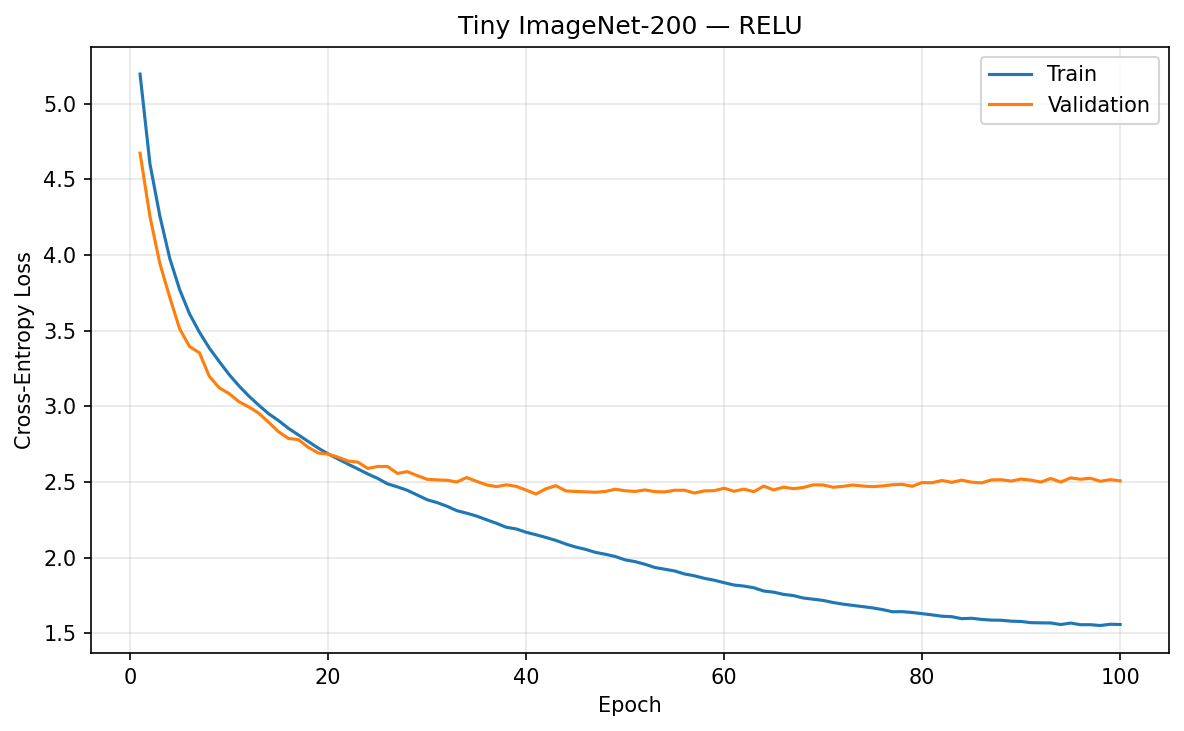
\includegraphics[width=\textwidth]{curves_train_relu.png}
    \caption{ReLU}
  \end{subfigure}
  \begin{subfigure}[b]{0.32\textwidth}
    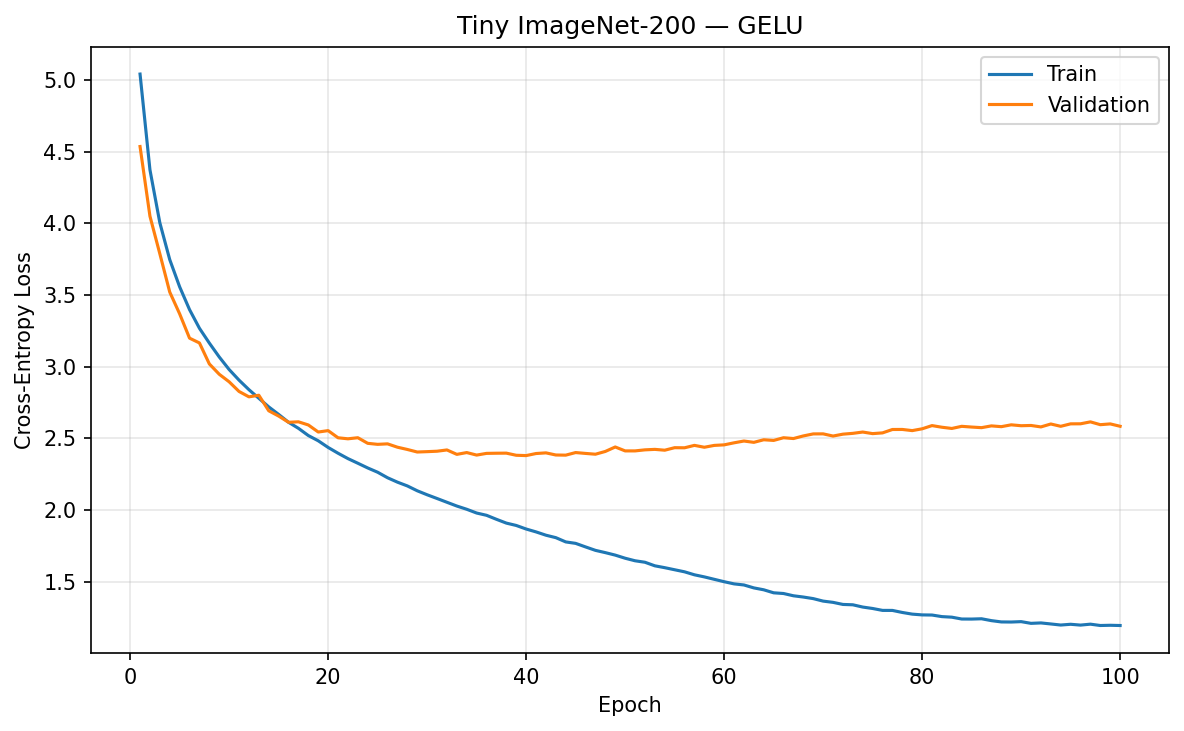
\includegraphics[width=\textwidth]{curves_train_gelu.png}
    \caption{GELU}
  \end{subfigure}
  \begin{subfigure}[b]{0.32\textwidth}
    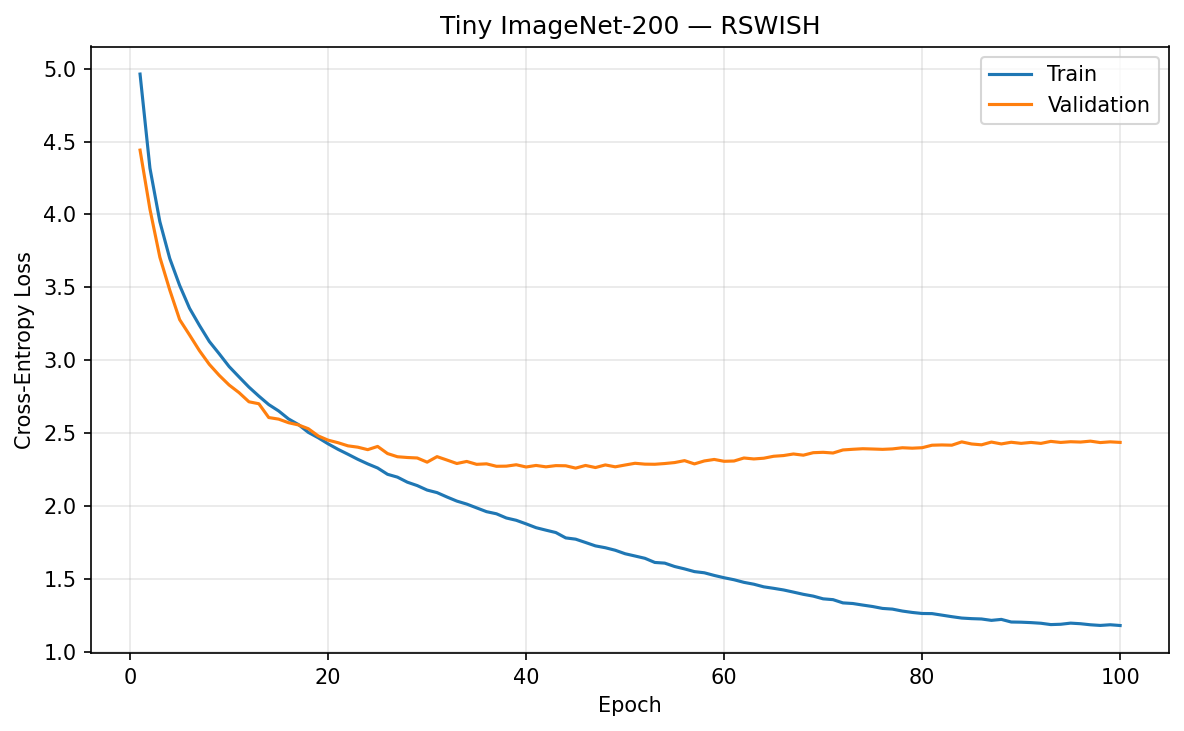
\includegraphics[width=\textwidth]{curves_train_rswish.png}
    \caption{RSwish}
  \end{subfigure}
  \caption{Train/validation loss curves on Tiny ImageNet-200 (100 epochs, batch 64).}
  \label{fig:curves_tiny}
\end{figure}

\subsection{Quantitative Evaluation Metrics --- Task~1 (Tiny ImageNet-200)}

Tables~\ref{tab:tiny_all} and~\ref{tab:tiny_conf} report full-coverage and
high-confidence metrics respectively.
All precision, recall, F1, and AUC values are macro-averaged across 200 classes.

\begin{table}[H]
  \centering
  \caption{Tiny ImageNet-200 test results --- full coverage (10{,}000 samples).
           Parameter counts: ResNet-18 $\approx$11.2M; CompactNet $\approx$1.1M.}
  \label{tab:tiny_all}
  \begin{tabular}{llcccccc}
    \toprule
    \textbf{Model} & \textbf{Activation} &
    \textbf{Acc (\%)} & \textbf{Prec (\%)} &
    \textbf{Recall (\%)} & \textbf{F1 (\%)} &
    \textbf{ROC-AUC} & \textbf{PR-AUC} \\
    \midrule
    ResNet-18 (baseline) & ReLU (built-in)
                    & 45.28 & 47.86 & 45.28 & 44.86 & 0.9678 & 0.4868 \\
    \midrule
    \multirow{3}{*}{CompactNet (proposed)}
                    & ReLU   & 42.87 & 42.90 & 42.87 & 42.23 & 0.9643 & 0.4426 \\
                    & GELU   & 45.10 & 45.39 & 45.10 & 44.71 & 0.9669 & 0.4718 \\
                    & \textbf{RSwish} & \textbf{47.83} & \textbf{48.17} & \textbf{47.83}
                    & \textbf{47.36} & \textbf{0.9701} & \textbf{0.5033} \\
    \bottomrule
  \end{tabular}
\end{table}

\begin{table}[H]
  \centering
  \caption{Tiny ImageNet-200 high-confidence results (max softmax $\geq 0.9$).}
  \label{tab:tiny_conf}
  \begin{tabular}{llcccccc}
    \toprule
    \textbf{Model} & \textbf{Activation} &
    \textbf{Acc (\%)} & \textbf{Prec (\%)} & \textbf{Recall (\%)} &
    \textbf{F1 (\%)} & \textbf{PR-AUC} & \textbf{Coverage (\%)} \\
    \midrule
    ResNet-18 (baseline) & ReLU (built-in)
                    & 90.10 & 81.25 & 77.46 & 77.74 & 0.7897 & 20.5 \\
    \midrule
    \multirow{3}{*}{CompactNet (proposed)}
                    & ReLU   & \textbf{92.32} & 83.19 & 80.41 & 80.90 & 0.7001 & 14.2 \\
                    & GELU   & 91.13 & 84.24 & 80.67 & 81.21 & 0.7759 & 18.0 \\
                    & \textbf{RSwish} & 91.29 & \textbf{85.03} & \textbf{82.56}
                    & \textbf{82.64} & \textbf{0.8157} & \textbf{21.5} \\
    \bottomrule
  \end{tabular}
\end{table}

RSwish leads on every full-coverage metric and on macro F1 and PR-AUC at the
confidence threshold.
Importantly, the RSwish model retains \textbf{21.5\%} of test samples above the
0.9 threshold---substantially more than ReLU (14.2\%) or GELU (18.0\%)---indicating
better-calibrated probability estimates overall.
ReLU achieves the highest raw accuracy among the high-confidence subset because it
is more conservative: it makes confident predictions only for the easiest examples.

Figure~\ref{fig:eval_tiny} shows the ROC curve, PR curve, and confusion matrix for
the best-performing RSwish model on Tiny ImageNet-200.

\begin{figure}[H]
  \centering
  \begin{subfigure}[b]{0.32\textwidth}
    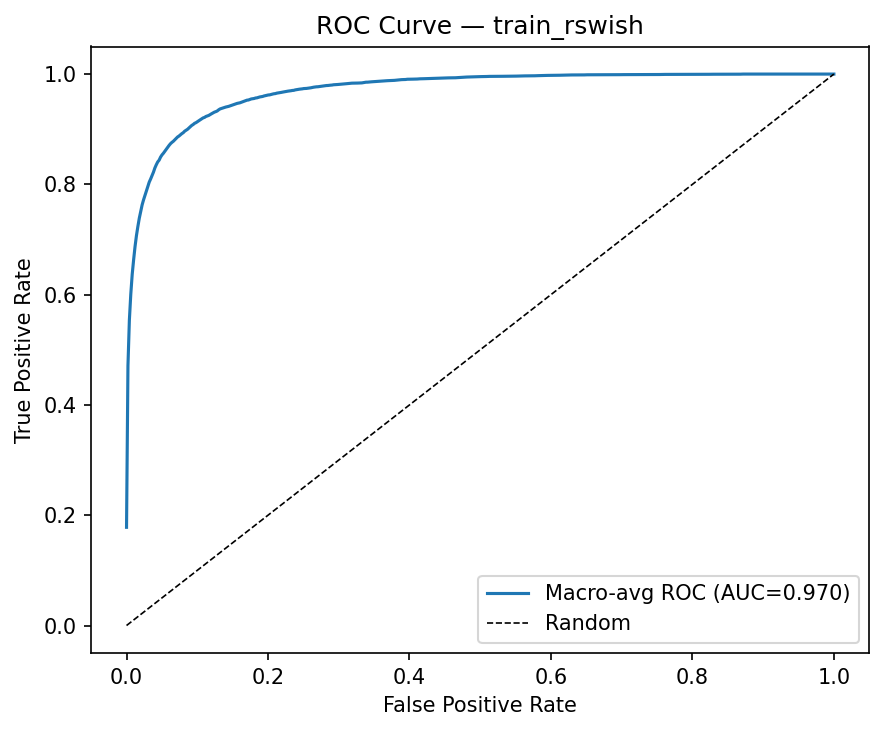
\includegraphics[width=\textwidth]{roc_train_rswish.png}
    \caption{ROC (macro-avg AUC = 0.970)}
  \end{subfigure}
  \begin{subfigure}[b]{0.32\textwidth}
    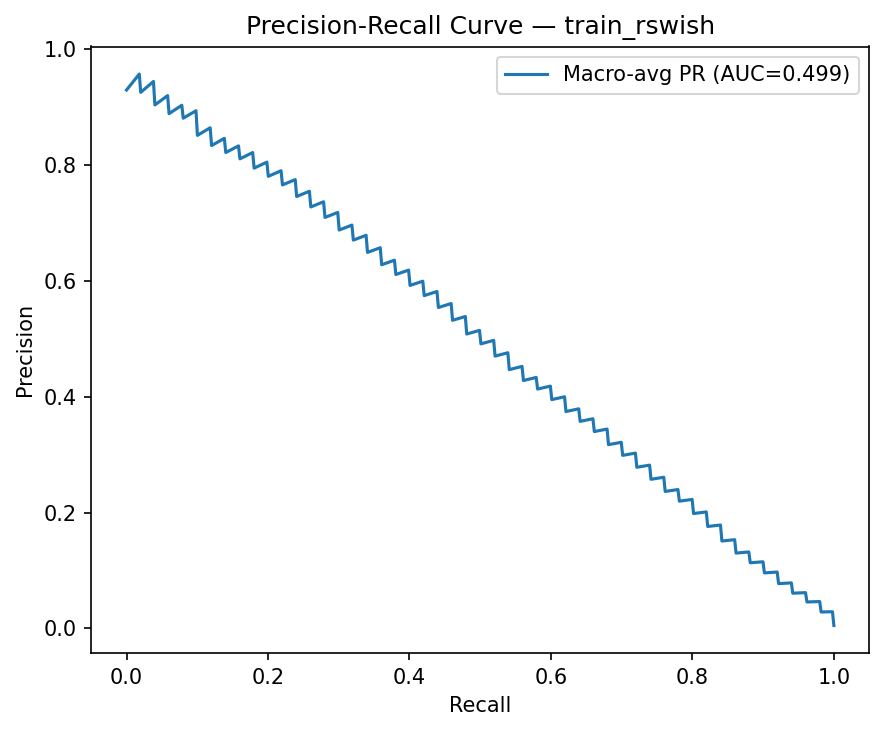
\includegraphics[width=\textwidth]{pr_train_rswish.png}
    \caption{Precision-Recall (macro-avg)}
  \end{subfigure}
  \begin{subfigure}[b]{0.32\textwidth}
    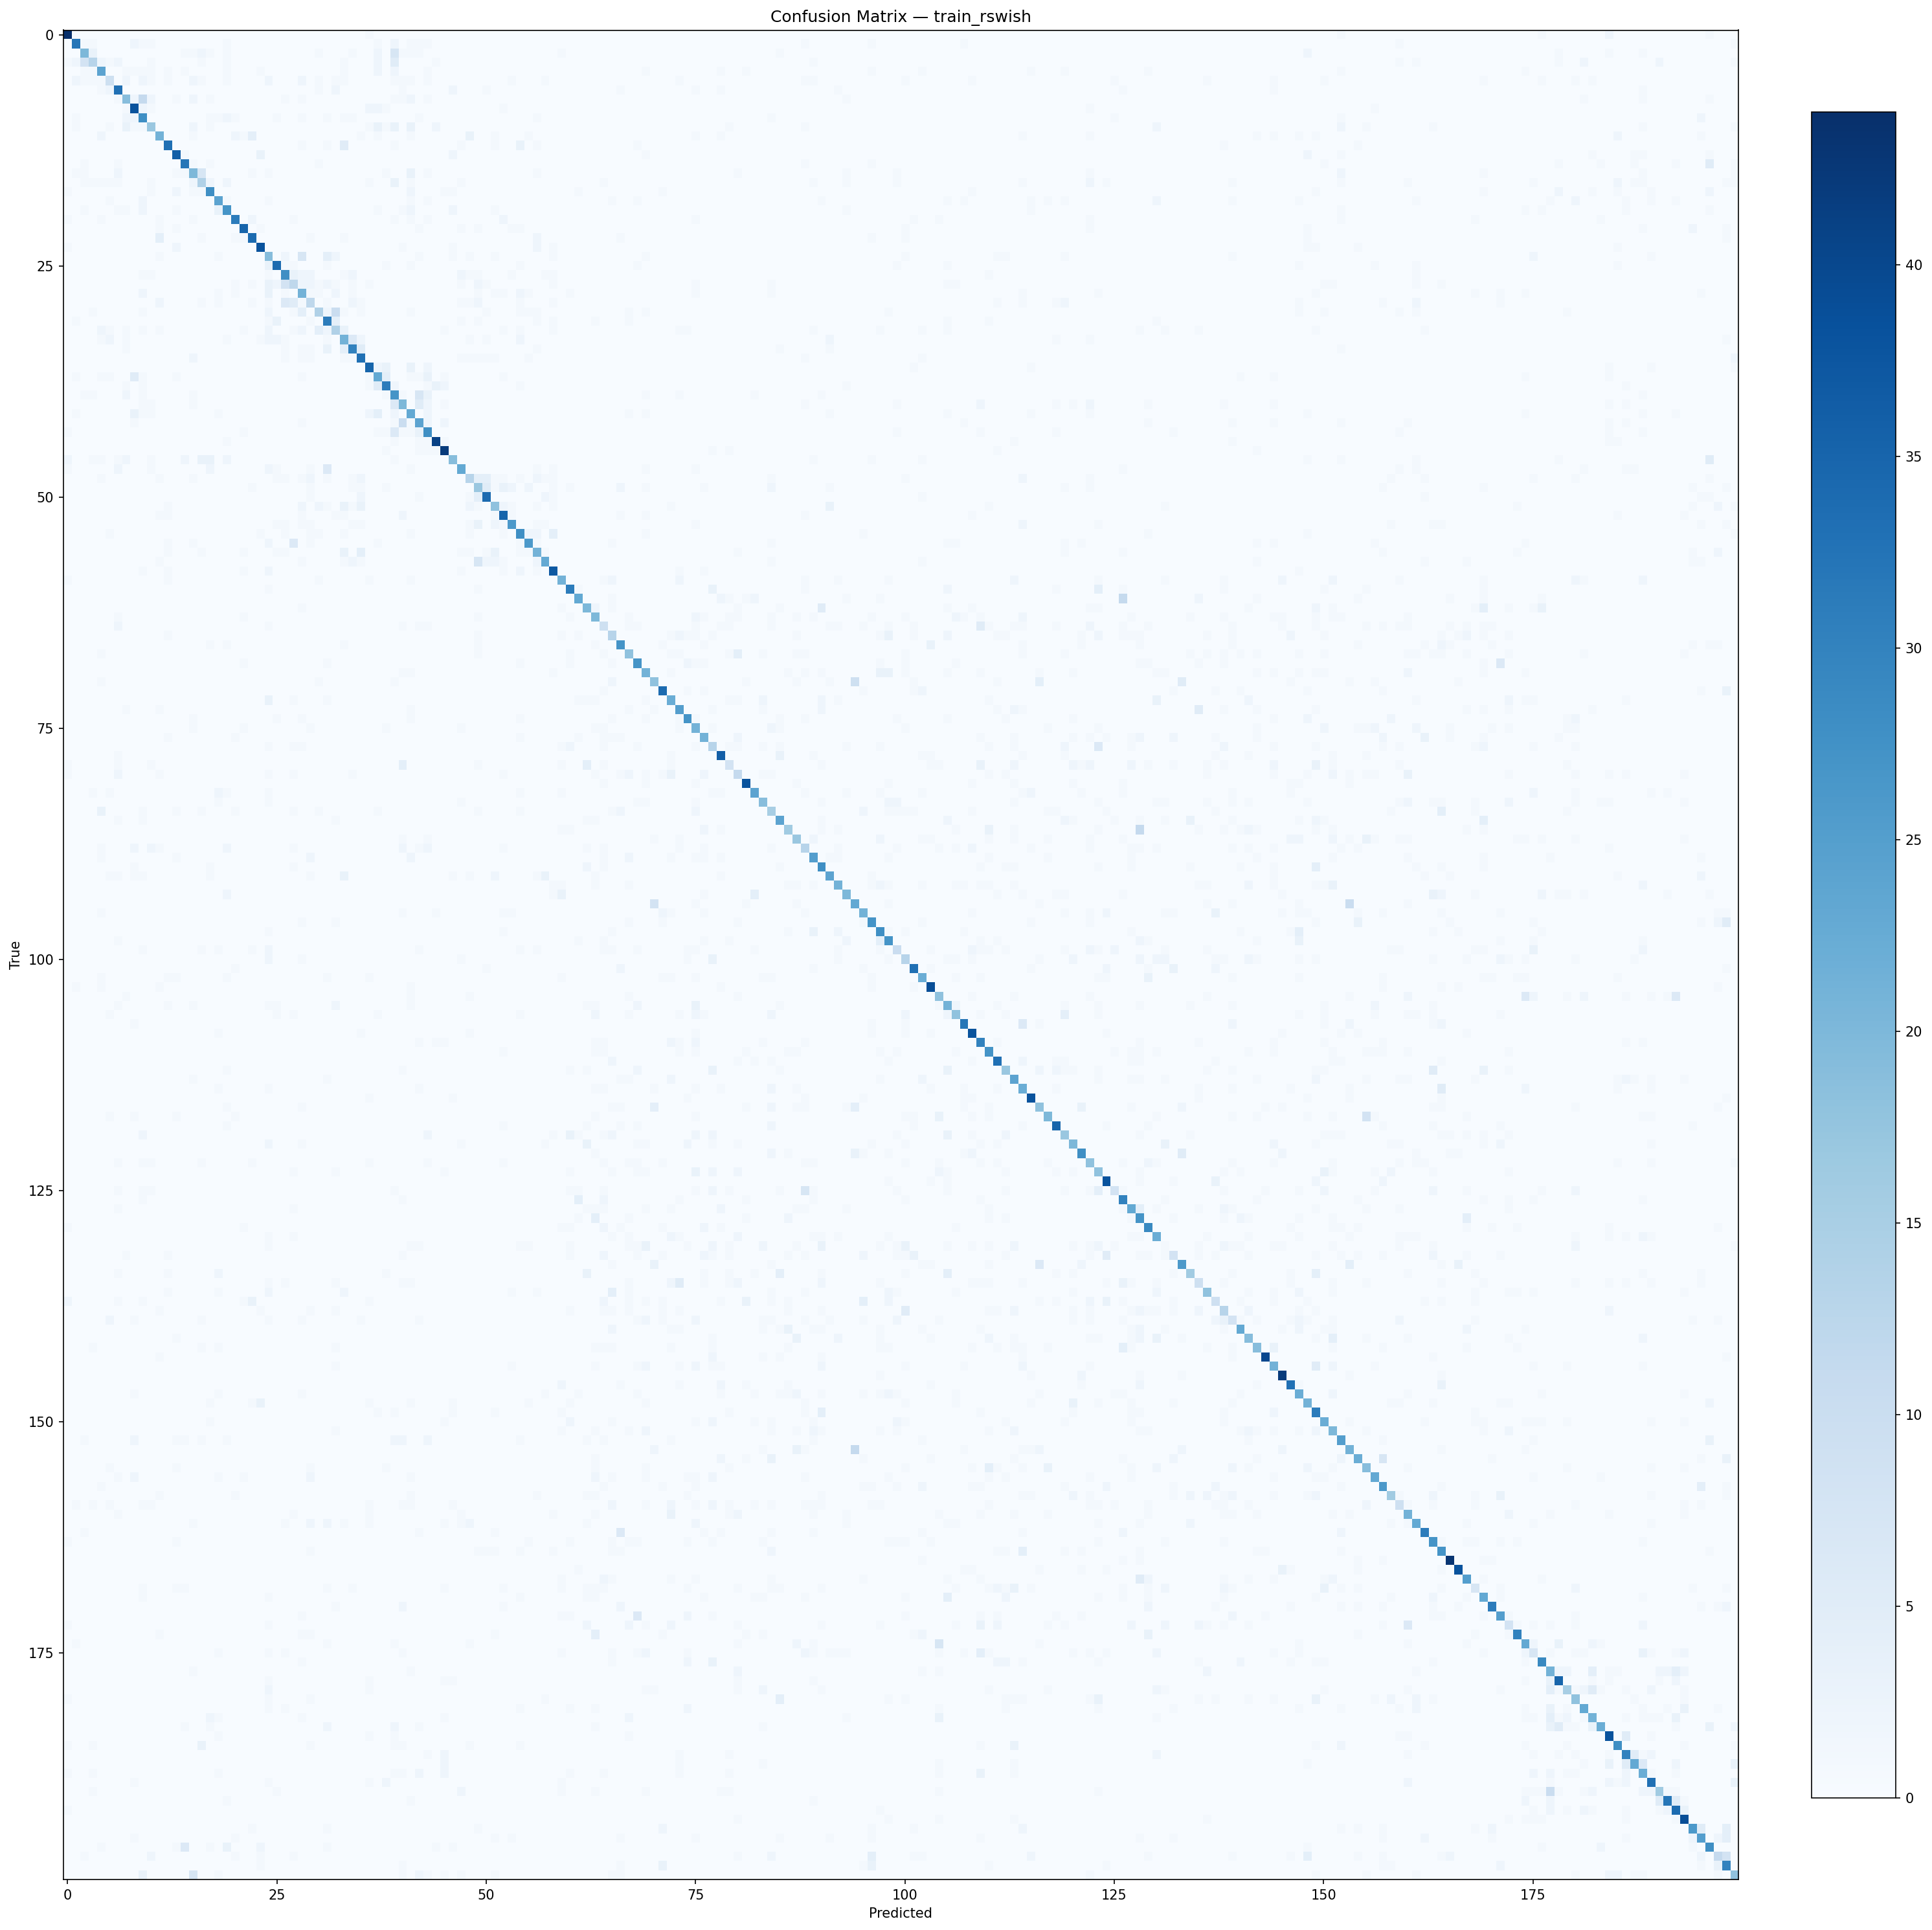
\includegraphics[width=\textwidth]{cm_train_rswish.png}
    \caption{Confusion matrix ($200\!\times\!200$)}
  \end{subfigure}
  \caption{Evaluation of the RSwish CompactNet on Tiny ImageNet-200 (full test set).}
  \label{fig:eval_tiny}
\end{figure}

\subsection{Training and Testing Performance --- Task~1 (CIFAR-100)}

RSwish was selected for all CIFAR-100 experiments.
Figure~\ref{fig:curves_cifar} shows the training curves for the from-scratch and
fine-tuned models over 50 epochs.
The fine-tuned model converges to a markedly lower validation loss (1.302 vs.\ 2.114),
confirming that Tiny ImageNet features transfer effectively to CIFAR-100.

\begin{figure}[H]
  \centering
  \begin{subfigure}[b]{0.48\textwidth}
    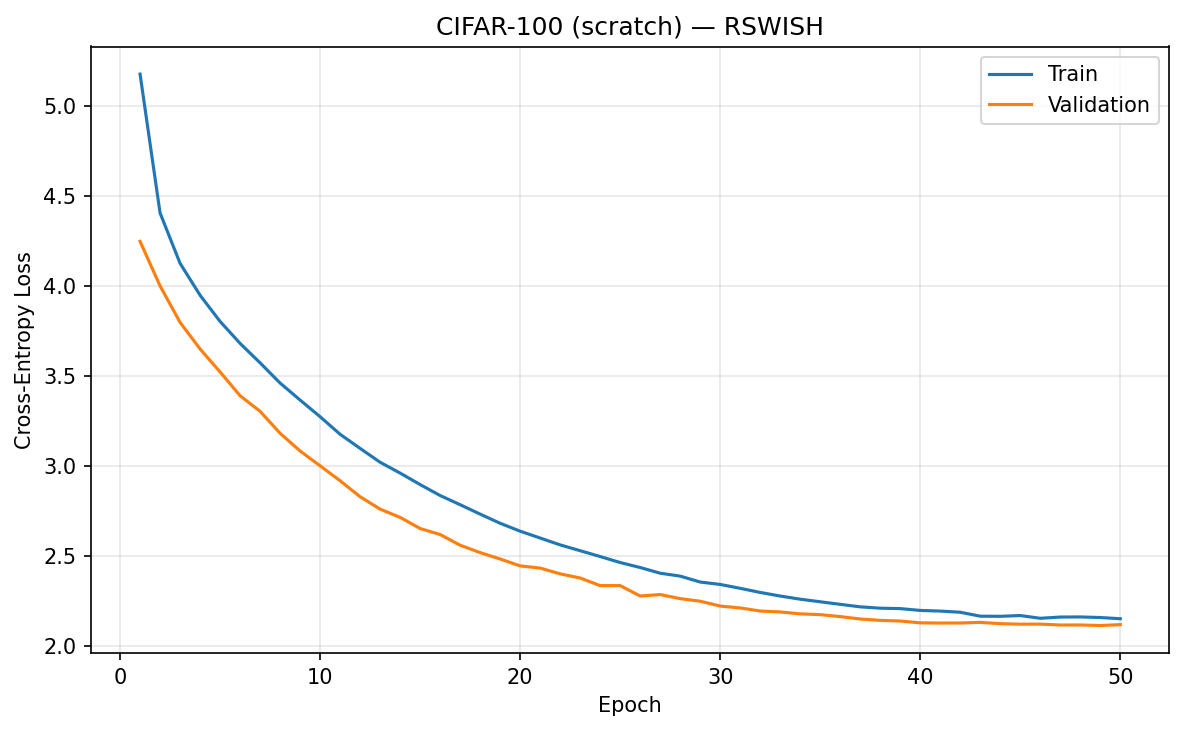
\includegraphics[width=\textwidth]{curves_scratch_rswish.png}
    \caption{From scratch (He init, val loss = 2.114)}
  \end{subfigure}
  \begin{subfigure}[b]{0.48\textwidth}
    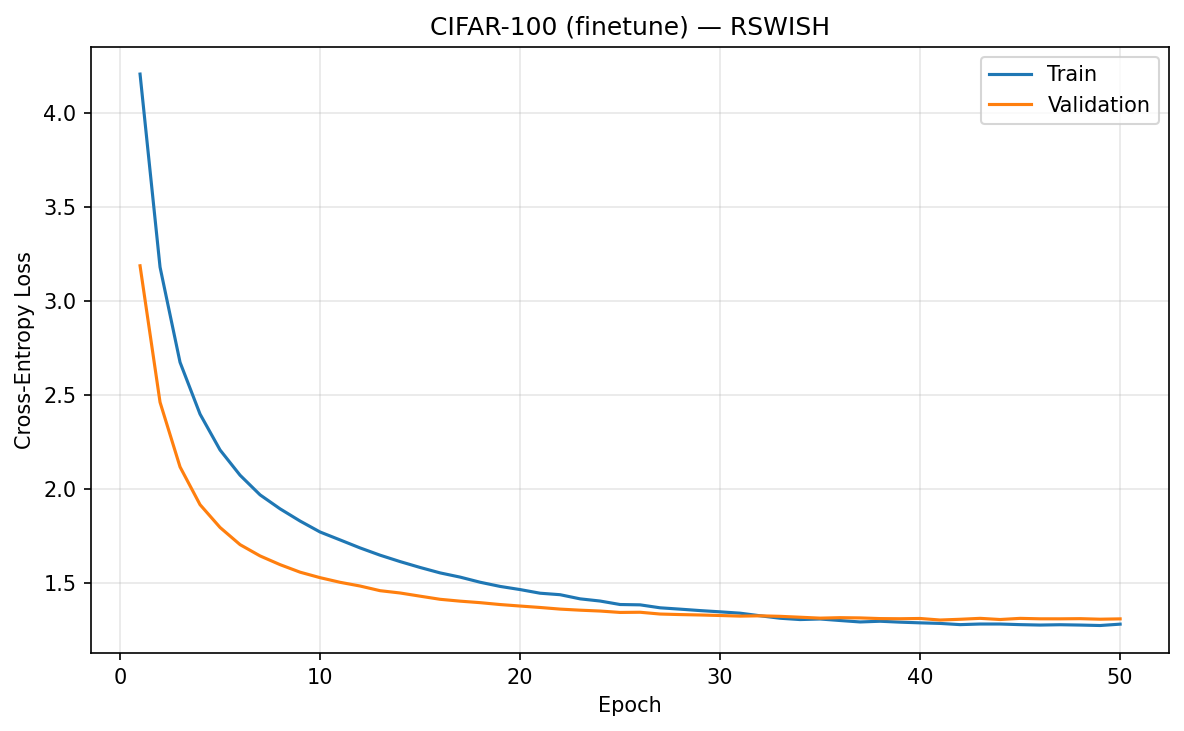
\includegraphics[width=\textwidth]{curves_finetune_rswish.png}
    \caption{Fine-tuned from Tiny ImageNet (val loss = 1.302)}
  \end{subfigure}
  \caption{Train/validation loss curves on CIFAR-100 (RSwish, 50 epochs, batch 64).}
  \label{fig:curves_cifar}
\end{figure}

\subsection{Training and Testing Performance --- Task~2 (Ensemble)}

Figure~\ref{fig:curves_ensemble} shows the per-member training curves for the
three-model ensemble.
Each member is initialised from the shared Tiny ImageNet checkpoint and fine-tuned
with a distinct random seed, inducing stochastic diversity in weight trajectories
while sharing a strong initialisation.

\begin{figure}[H]
  \centering
  \begin{subfigure}[b]{0.32\textwidth}
    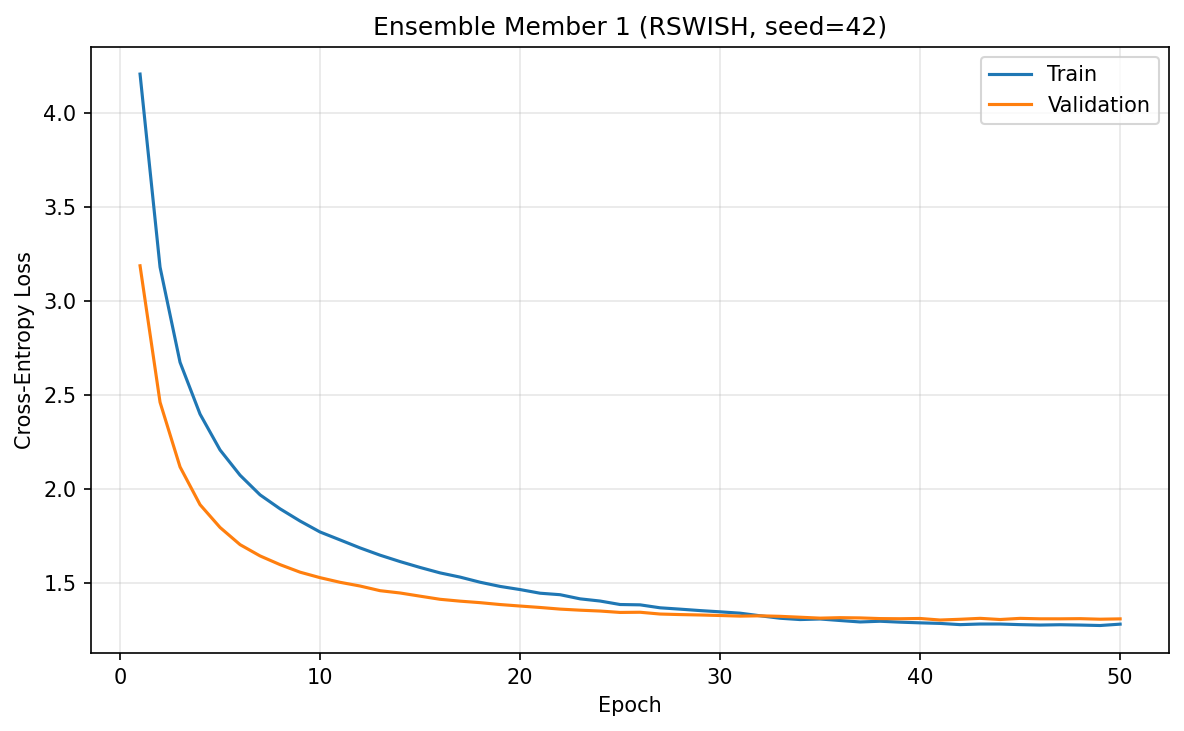
\includegraphics[width=\textwidth]{curves_ensemble_rswish_seed42.png}
    \caption{Member 1 (seed 42)}
  \end{subfigure}
  \begin{subfigure}[b]{0.32\textwidth}
    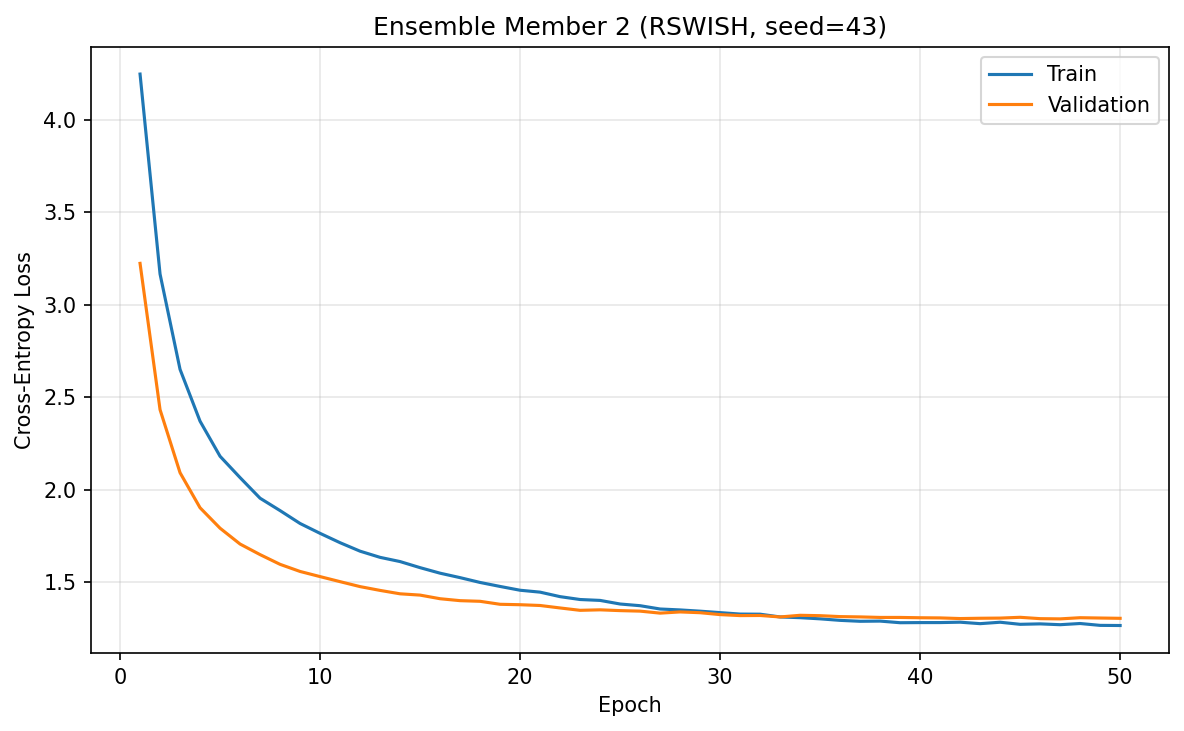
\includegraphics[width=\textwidth]{curves_ensemble_rswish_seed43.png}
    \caption{Member 2 (seed 43)}
  \end{subfigure}
  \begin{subfigure}[b]{0.32\textwidth}
    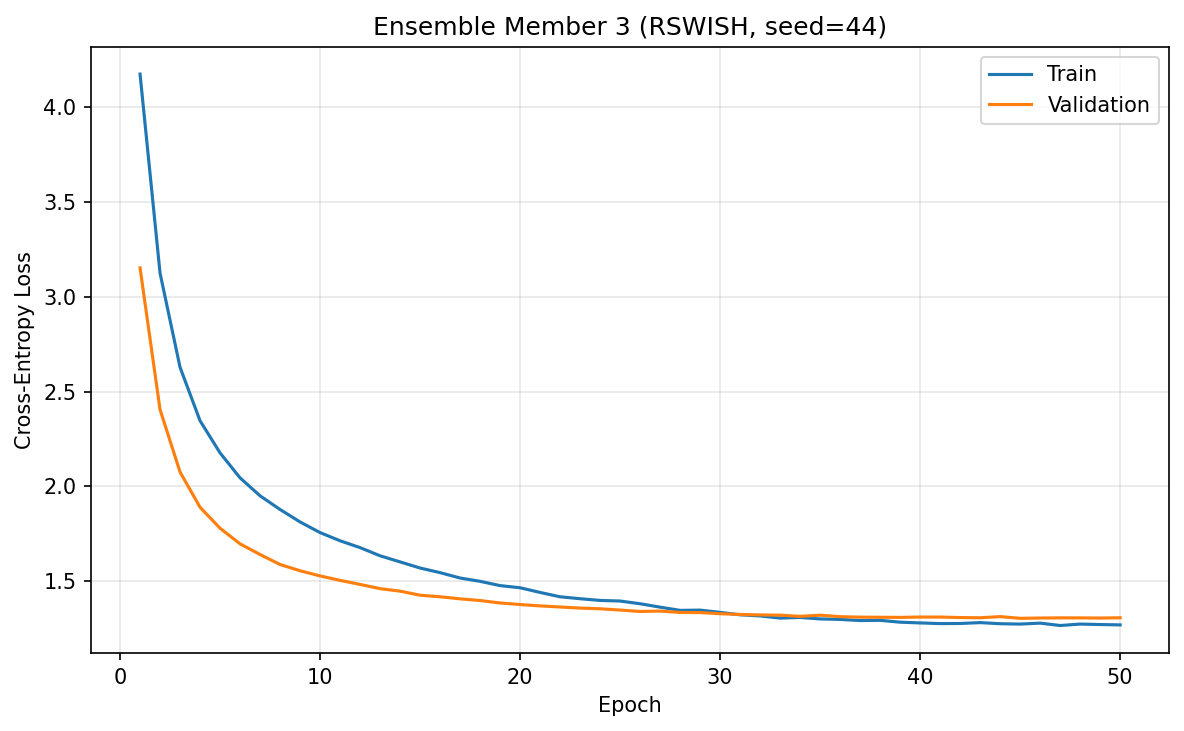
\includegraphics[width=\textwidth]{curves_ensemble_rswish_seed44.png}
    \caption{Member 3 (seed 44)}
  \end{subfigure}
  \caption{Per-member training curves for the RSwish ensemble on CIFAR-100.}
  \label{fig:curves_ensemble}
\end{figure}

\subsection{Quantitative Evaluation Metrics --- CIFAR-100}

Table~\ref{tab:cifar_all} compares all three CIFAR-100 conditions at full coverage;
Table~\ref{tab:cifar_conf} shows high-confidence results.
Ensemble combination uses soft voting: the three members' softmax distributions are
averaged before the argmax decision.

\begin{table}[H]
  \centering
  \caption{CIFAR-100 test results --- full coverage (10{,}000 samples, RSwish).}
  \label{tab:cifar_all}
  \begin{tabular}{lcccccc}
    \toprule
    \textbf{Method} &
    \textbf{Acc (\%)} & \textbf{Prec (\%)} &
    \textbf{Recall (\%)} & \textbf{F1 (\%)} &
    \textbf{ROC-AUC} & \textbf{PR-AUC} \\
    \midrule
    Scratch              & 44.63 & 44.02 & 44.63 & 43.91 & 0.9598 & 0.4562 \\
    Fine-tune            & 63.35 & 63.15 & 63.35 & 63.09 & 0.9868 & 0.6889 \\
    \textbf{Ensemble (3$\times$)} & \textbf{64.65} & \textbf{64.47} & \textbf{64.65}
                         & \textbf{64.39} & \textbf{0.9884} & \textbf{0.7086} \\
    \bottomrule
  \end{tabular}
\end{table}

\begin{table}[H]
  \centering
  \caption{CIFAR-100 high-confidence results (max softmax $\geq 0.9$, RSwish).}
  \label{tab:cifar_conf}
  \begin{tabular}{lccccc}
    \toprule
    \textbf{Method} &
    \textbf{Acc (\%)} & \textbf{F1 (\%)} &
    \textbf{PR-AUC} & \textbf{Coverage (\%)} \\
    \midrule
    Scratch              & 93.43 & 74.32 & 0.6371 & 10.8 \\
    Fine-tune            & 95.22 & 91.73 & 0.8842 & 29.7 \\
    \textbf{Ensemble (3$\times$)} & \textbf{96.32} & \textbf{93.37} & \textbf{0.9062} & 28.0 \\
    \bottomrule
  \end{tabular}
\end{table}

Figures~\ref{fig:eval_finetune} and~\ref{fig:eval_ensemble} show the ROC, PR, and
confusion-matrix plots for the fine-tuned single model and the ensemble,
respectively.

\begin{figure}[H]
  \centering
  \begin{subfigure}[b]{0.32\textwidth}
    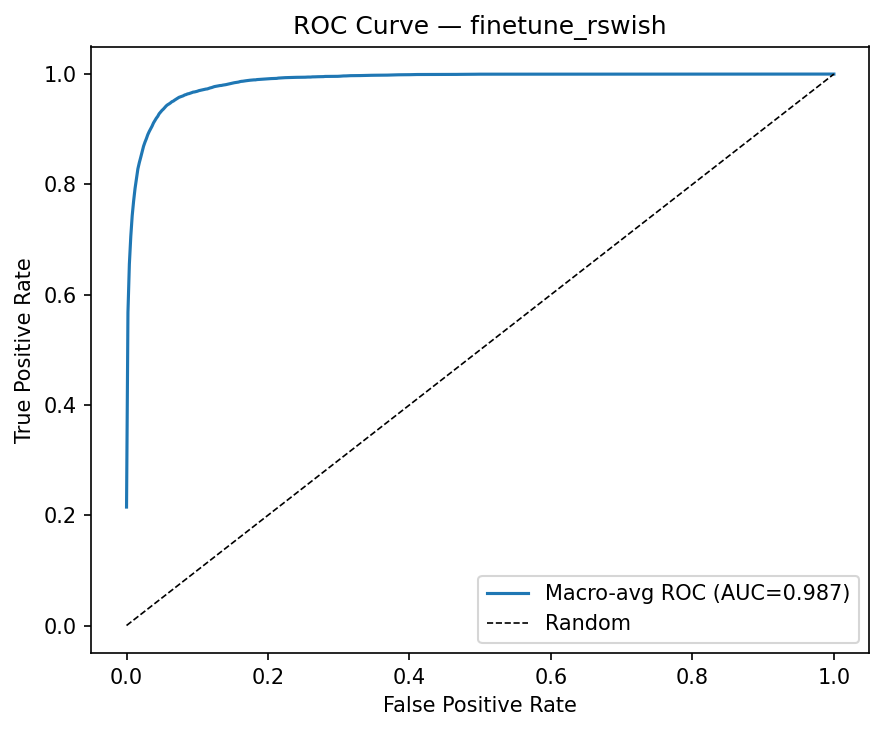
\includegraphics[width=\textwidth]{roc_finetune_rswish.png}
    \caption{ROC (AUC = 0.987)}
  \end{subfigure}
  \begin{subfigure}[b]{0.32\textwidth}
    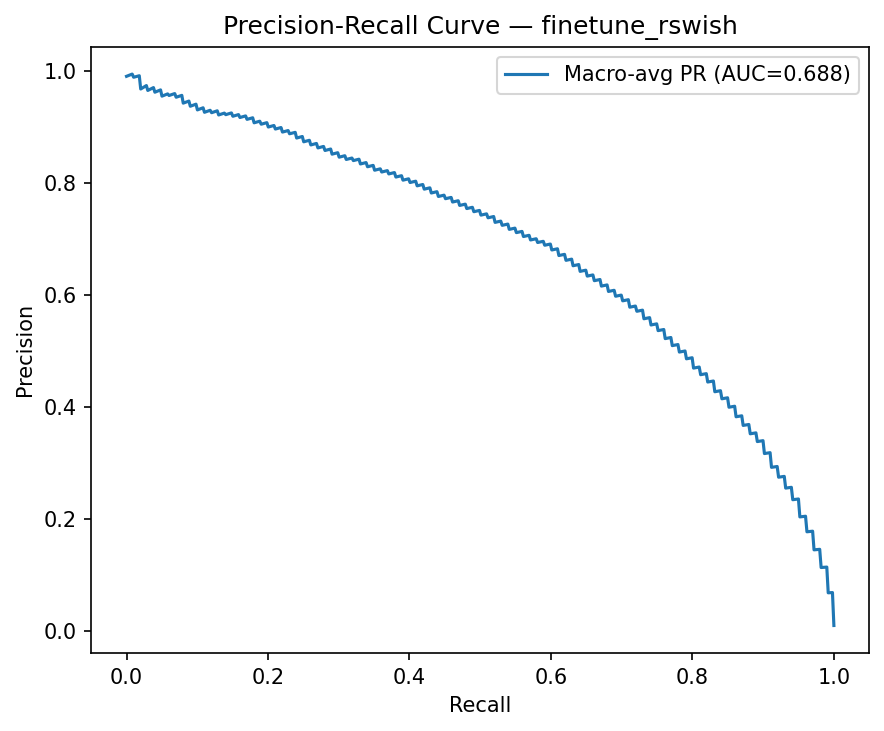
\includegraphics[width=\textwidth]{pr_finetune_rswish.png}
    \caption{Precision-Recall}
  \end{subfigure}
  \begin{subfigure}[b]{0.32\textwidth}
    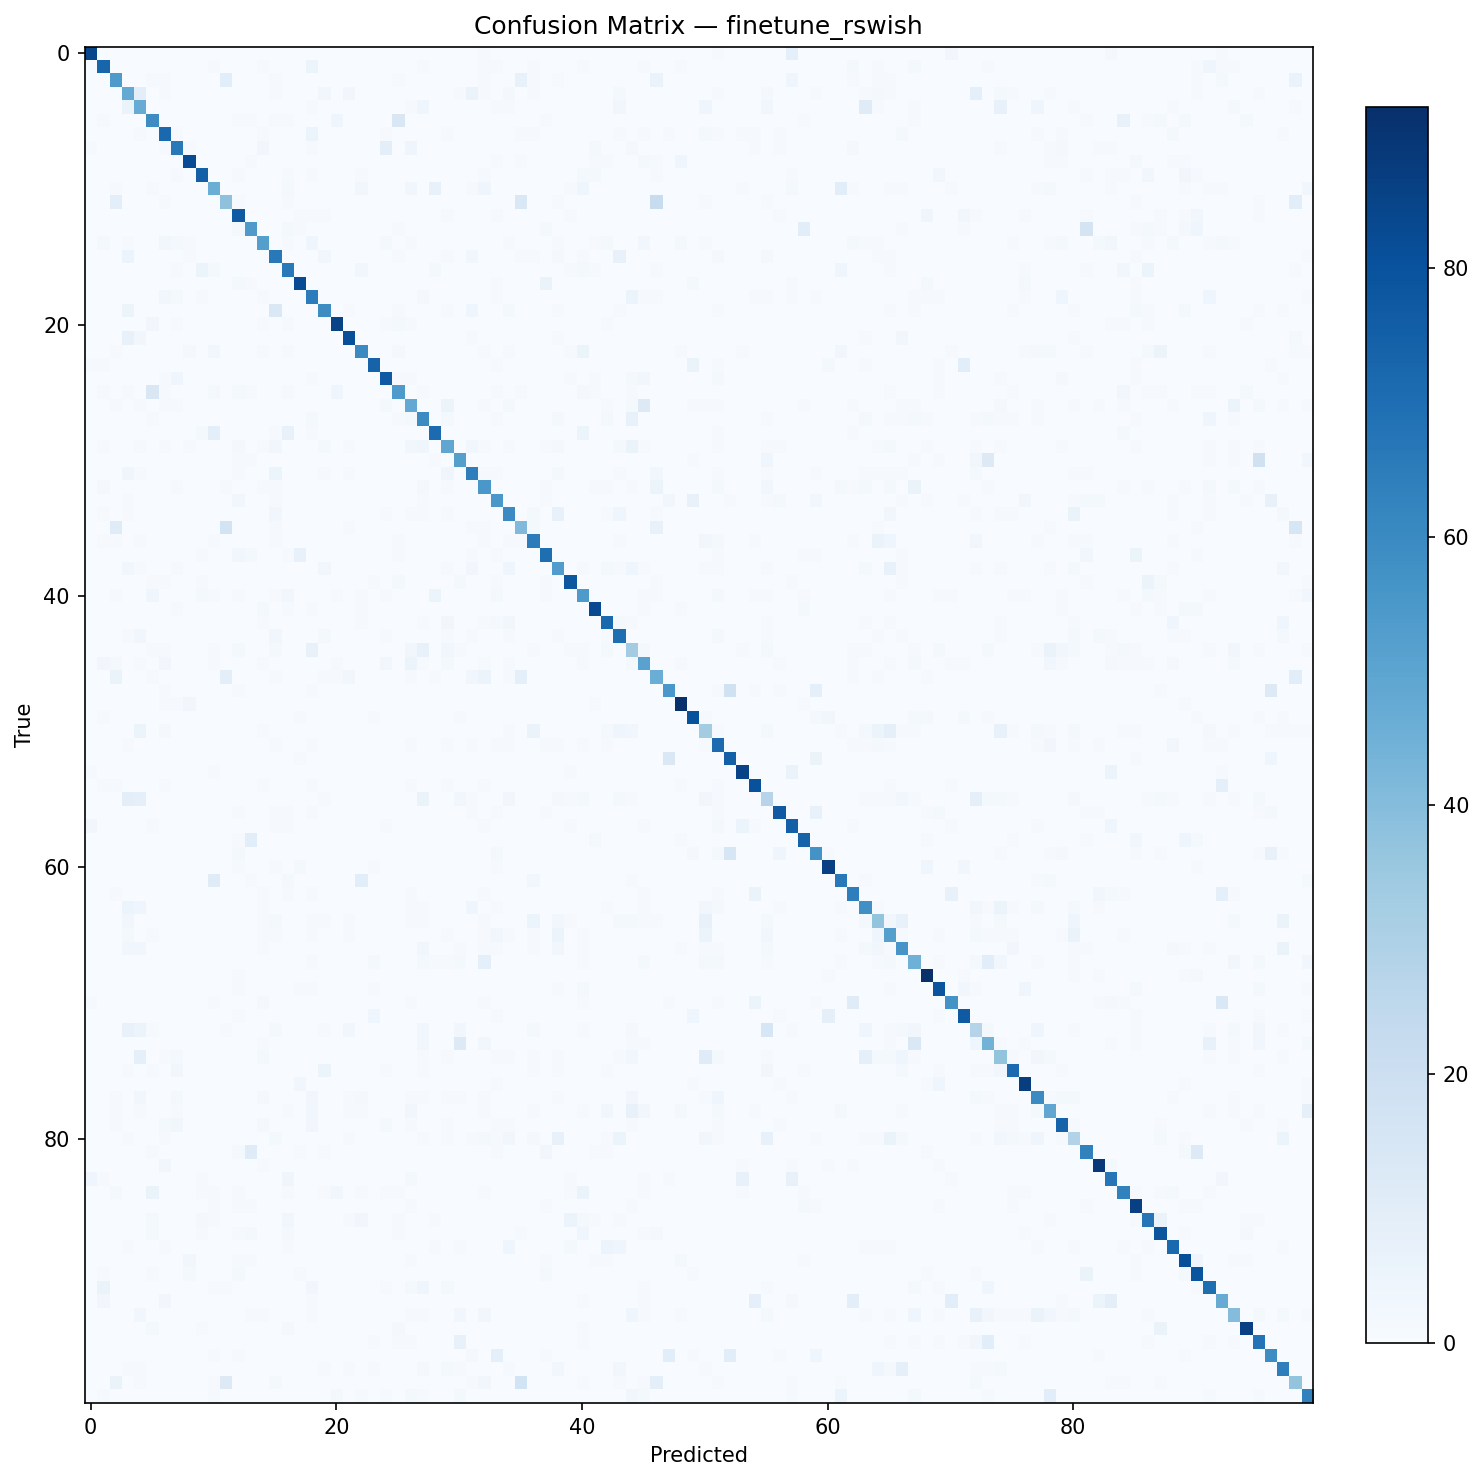
\includegraphics[width=\textwidth]{cm_finetune_rswish.png}
    \caption{Confusion matrix ($100\!\times\!100$)}
  \end{subfigure}
  \caption{Fine-tuned RSwish CompactNet on CIFAR-100 (full test set).}
  \label{fig:eval_finetune}
\end{figure}

\begin{figure}[H]
  \centering
  \begin{subfigure}[b]{0.32\textwidth}
    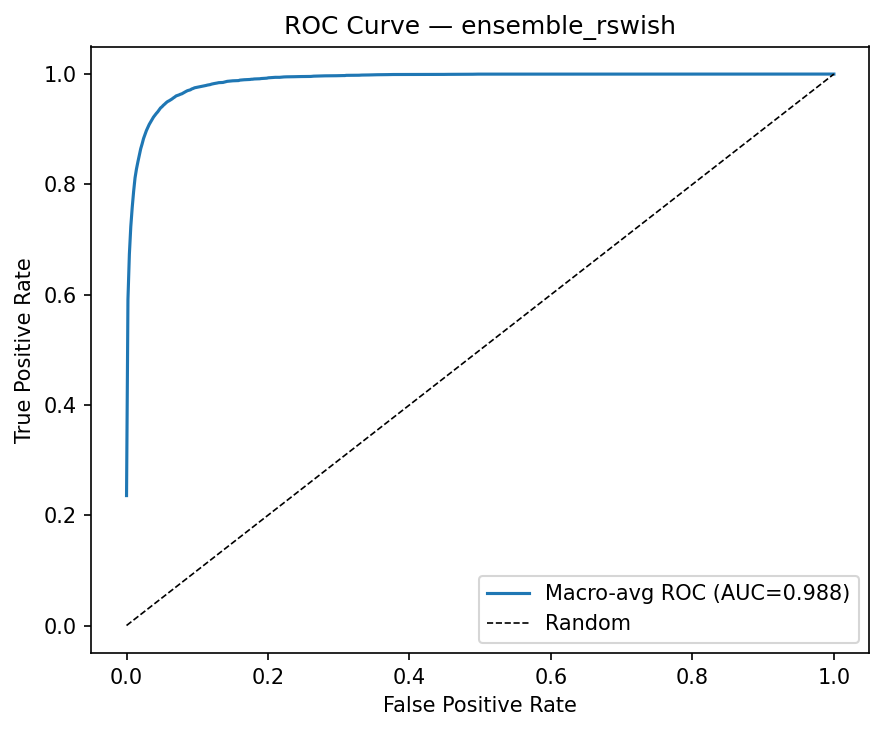
\includegraphics[width=\textwidth]{roc_ensemble_rswish.png}
    \caption{ROC (AUC = 0.988)}
  \end{subfigure}
  \begin{subfigure}[b]{0.32\textwidth}
    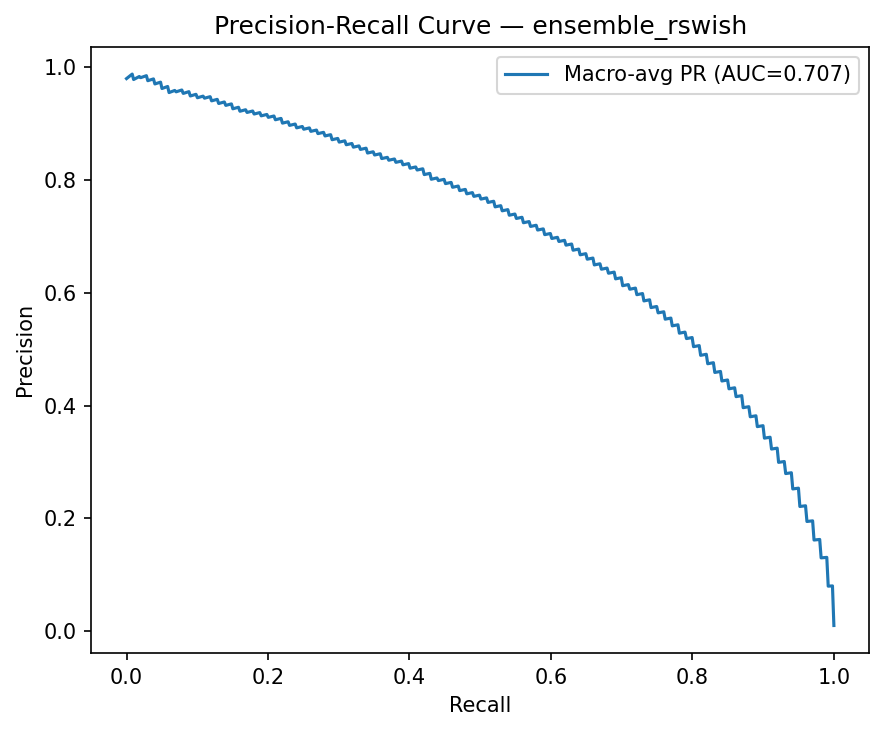
\includegraphics[width=\textwidth]{pr_ensemble_rswish.png}
    \caption{Precision-Recall}
  \end{subfigure}
  \begin{subfigure}[b]{0.32\textwidth}
    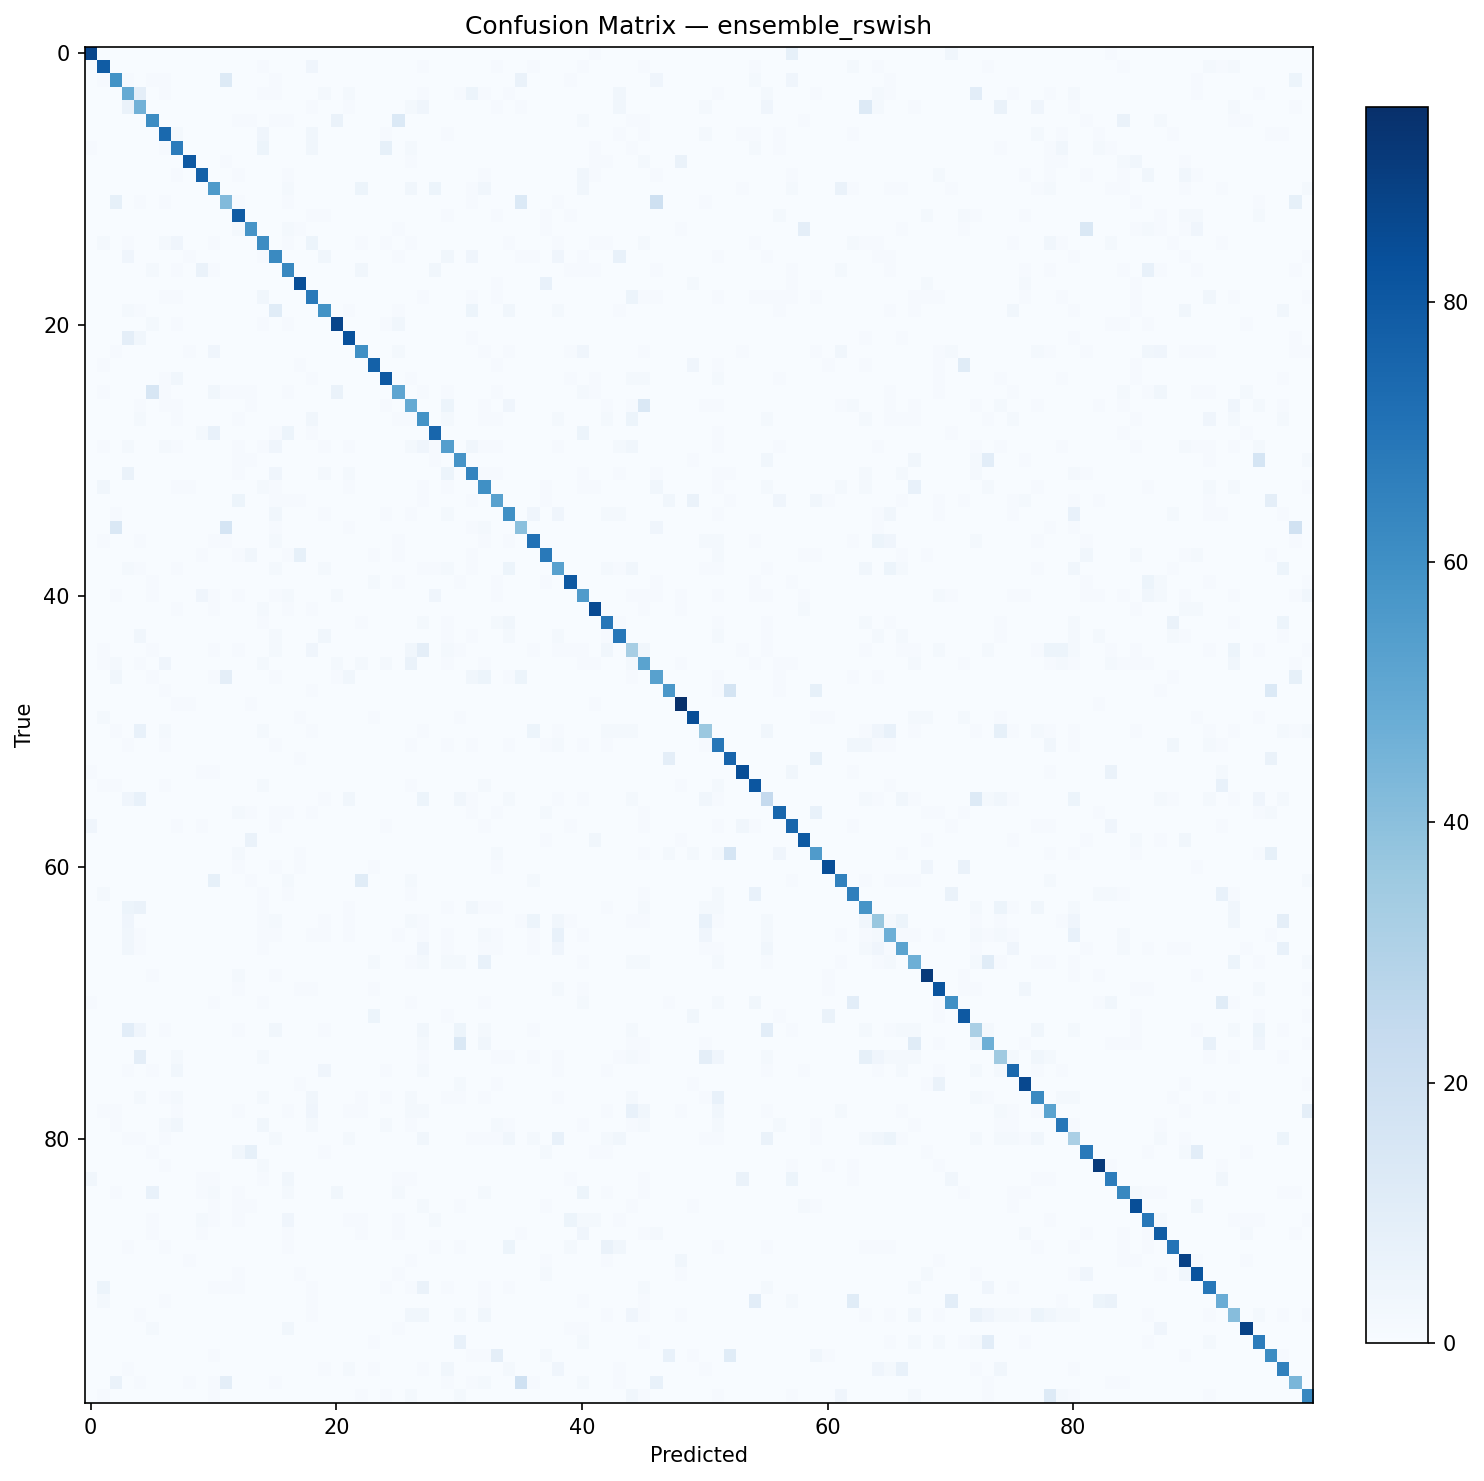
\includegraphics[width=\textwidth]{cm_ensemble_rswish.png}
    \caption{Confusion matrix ($100\!\times\!100$)}
  \end{subfigure}
  \caption{Three-model RSwish ensemble on CIFAR-100 (full test set).}
  \label{fig:eval_ensemble}
\end{figure}

Figure~\ref{fig:conf90} shows the confusion matrices restricted to predictions
with confidence $\geq 0.9$, confirming the strong diagonal dominance that
characterises high-confidence predictions.

\begin{figure}[H]
  \centering
  \begin{subfigure}[b]{0.48\textwidth}
    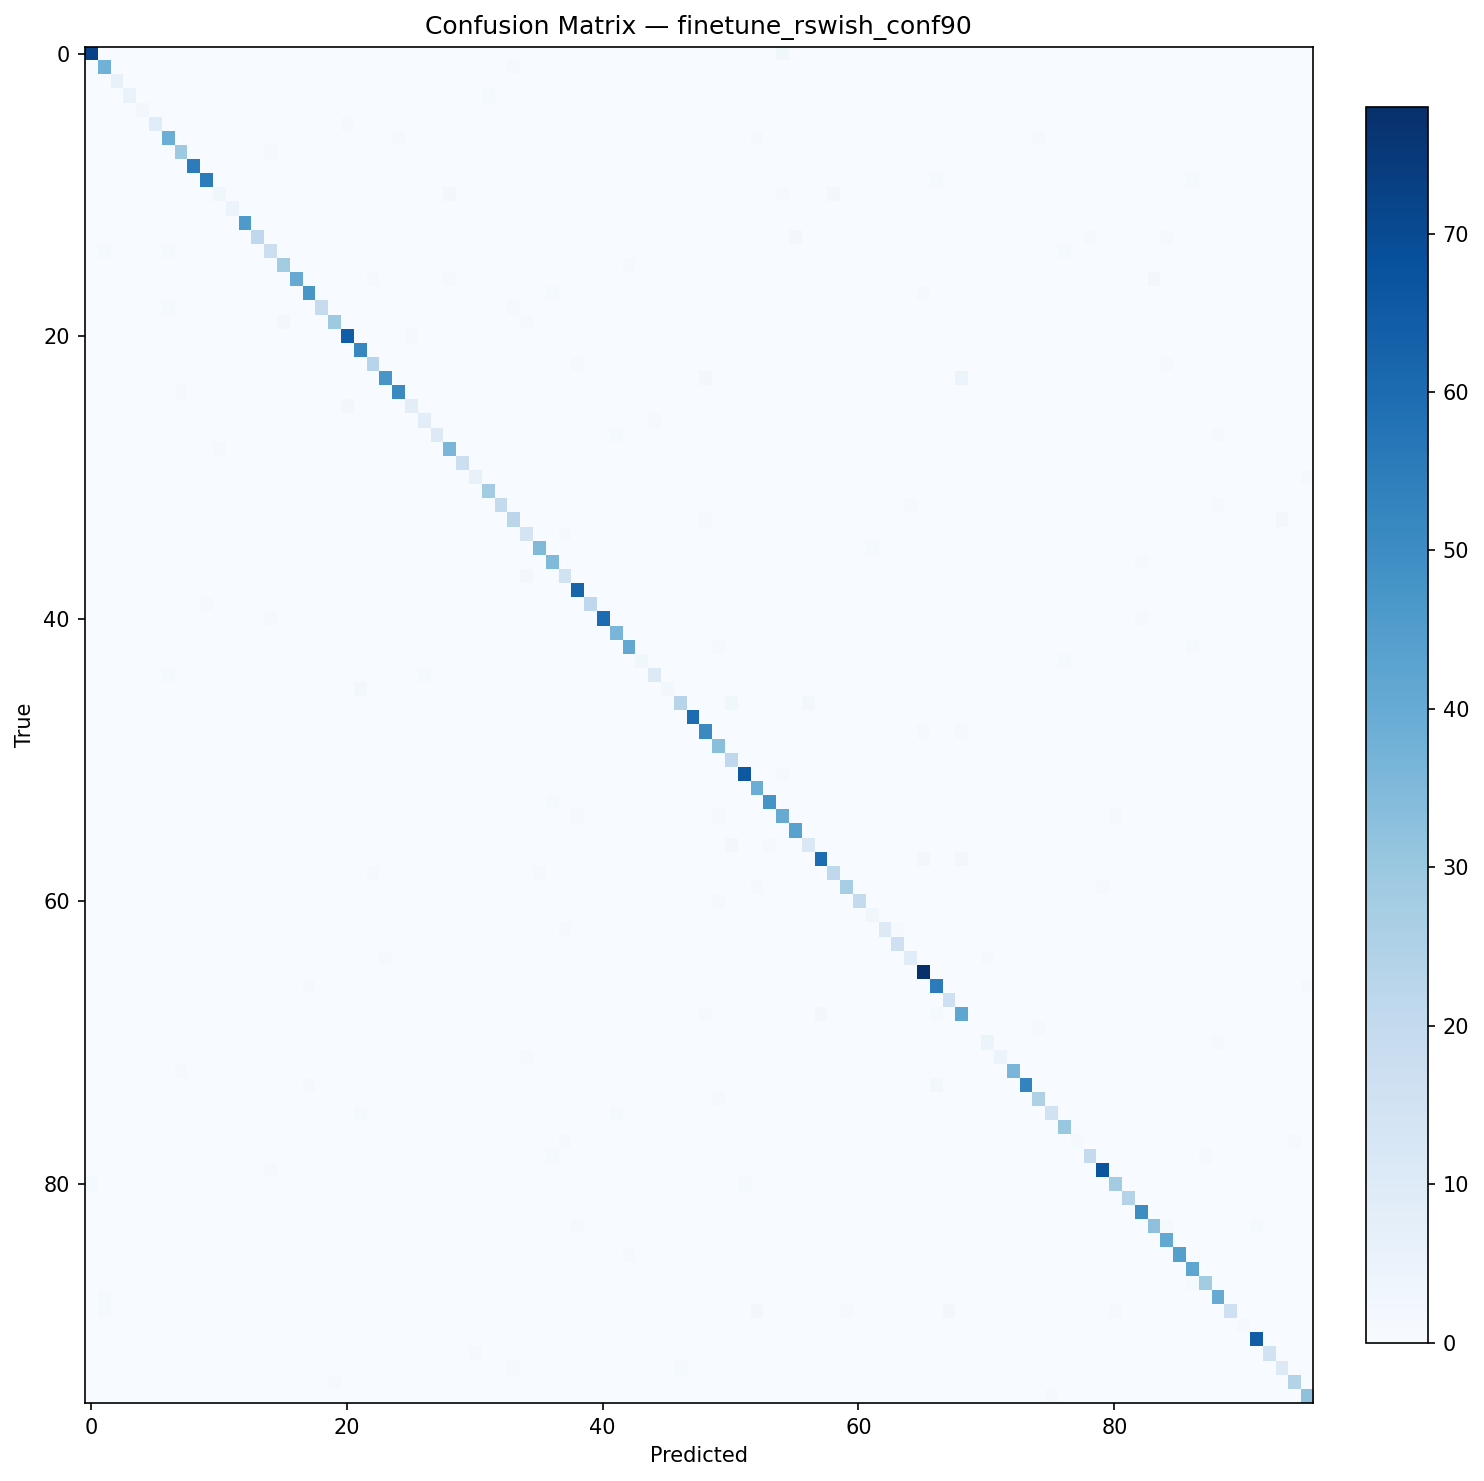
\includegraphics[width=\textwidth]{cm_finetune_rswish_conf90.png}
    \caption{Fine-tune (coverage 29.7\%, acc 95.22\%)}
  \end{subfigure}
  \begin{subfigure}[b]{0.48\textwidth}
    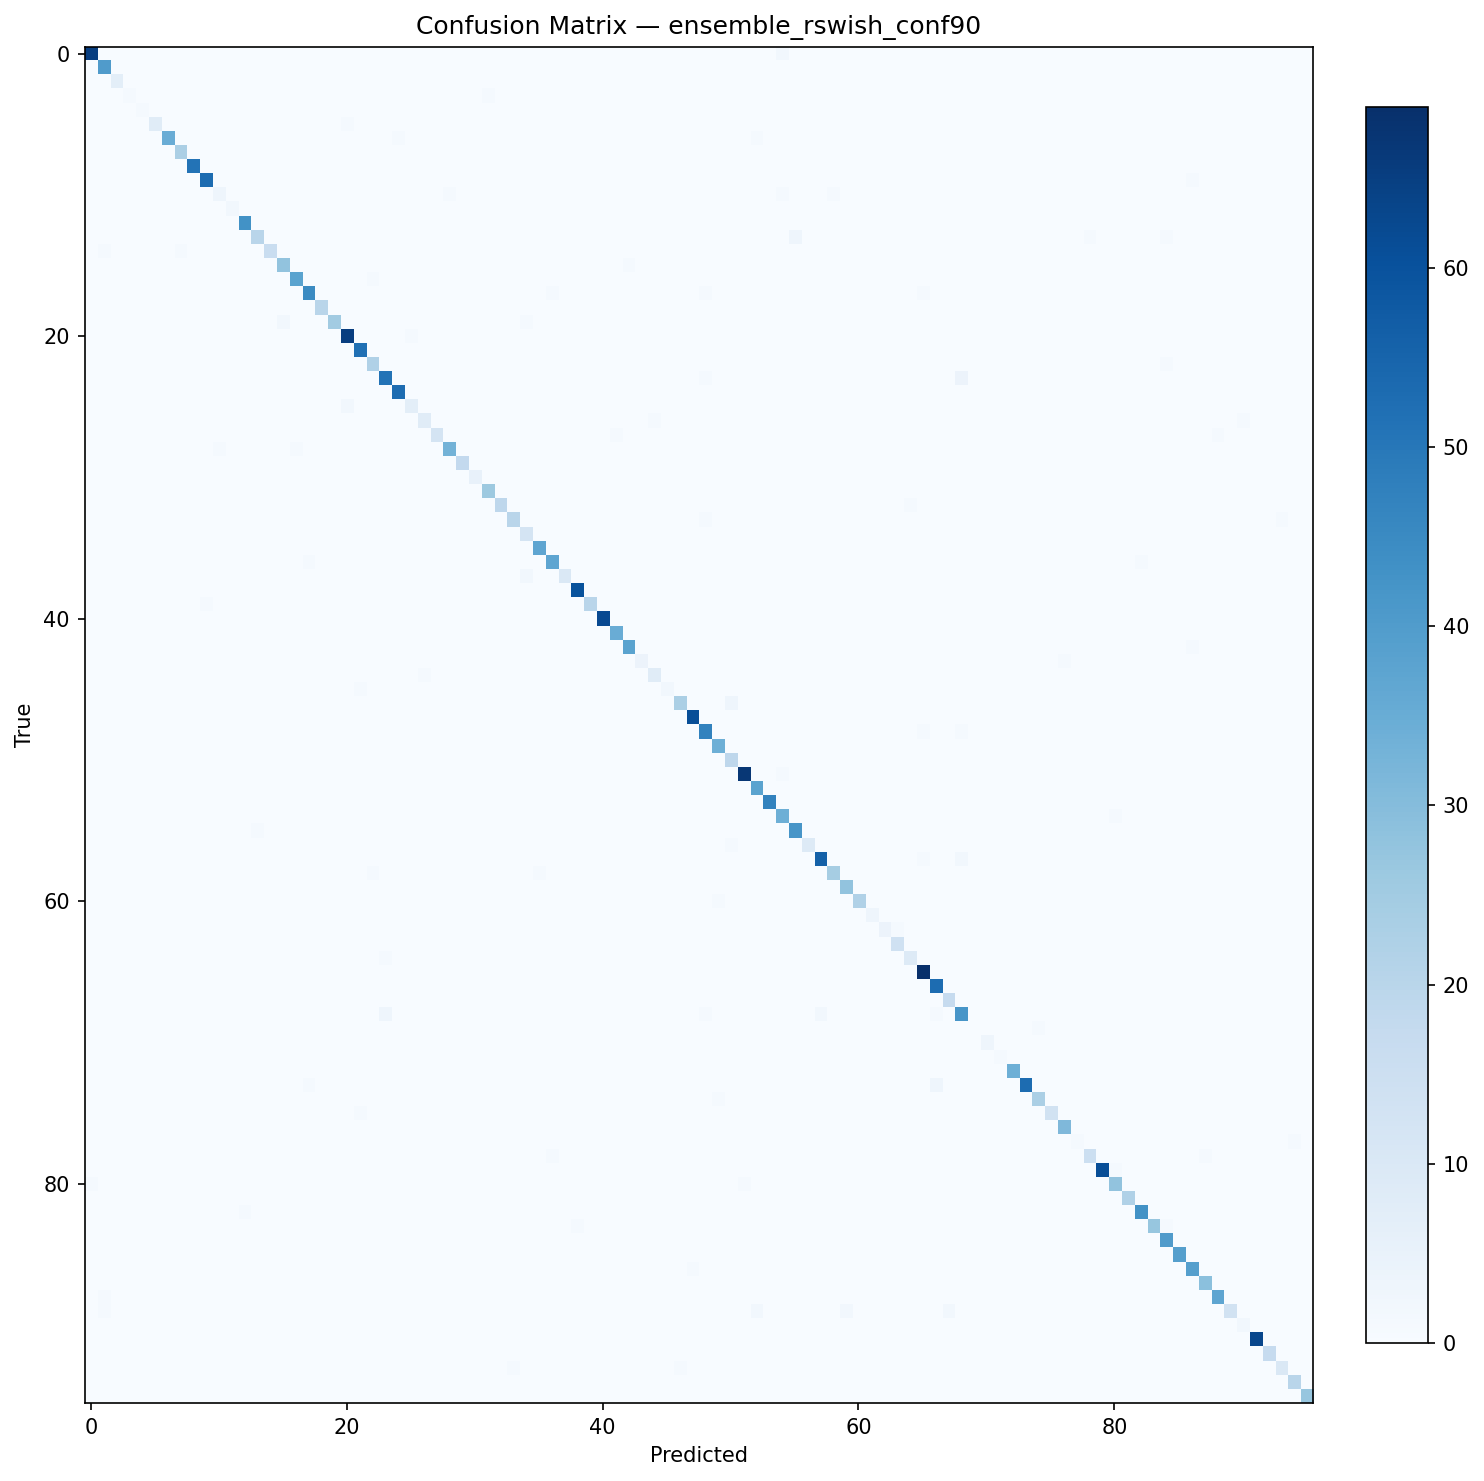
\includegraphics[width=\textwidth]{cm_ensemble_rswish_conf90.png}
    \caption{Ensemble (coverage 28.0\%, acc 96.32\%)}
  \end{subfigure}
  \caption{Confusion matrices for high-confidence predictions ($\geq 0.9$) on
           CIFAR-100.}
  \label{fig:conf90}
\end{figure}

\subsection{Comparative Analysis}

\paragraph{Baseline comparison and activation function analysis (Tiny ImageNet-200).}
Table~\ref{tab:tiny_all} compares all models at full coverage.
ResNet-18~\cite{he2016deep}, the standard reference architecture with $\approx$11.2M
parameters, achieves 45.28\% accuracy.
CompactNet with RSwish reaches \textbf{47.83\%}---a \textbf{+2.55 pp} gain over
ResNet-18 using approximately \textbf{11$\times$ fewer parameters} ($\approx$1.1M
vs.\ $\approx$11.2M).
CompactNet with ReLU (42.87\%) falls below ResNet-18, and GELU (45.10\%) is
marginally below it, confirming that the performance gain over the baseline is
specifically attributable to the RSwish activation rather than the bottleneck
architecture alone.
At the high-confidence threshold (Table~\ref{tab:tiny_conf}), all CompactNet variants
outperform ResNet-18 in F1 and PR-AUC, with RSwish achieving the highest scores across
every metric.
The rational sigmoid gate is smooth (avoiding the dead-neuron pathology of ReLU) and
avoids transcendental operations (unlike GELU's error function), making it both more
expressive and computationally comparable to ReLU.
RSwish achieves a 4.96 pp gain over CompactNet-ReLU and a 2.73 pp gain over
CompactNet-GELU in accuracy.

\paragraph{Transfer learning benefit (CIFAR-100).}
Fine-tuning from Tiny ImageNet pre-trained weights yields a \textbf{+18.7 pp}
accuracy improvement over training from scratch (63.35\% vs.\ 44.63\%).
This large gain over just 50 fine-tuning epochs confirms that the 200-class Tiny
ImageNet features---encoding edges, textures, and object parts at multiple
scales---generalise effectively to the 100-class CIFAR-100 domain.
The ROC-AUC gain (0.9598 $\to$ 0.9868) and PR-AUC gain (0.4562 $\to$ 0.6889)
further demonstrate improved discriminability across all classes.

\paragraph{Ensemble benefit (CIFAR-100).}
Soft voting over three independently fine-tuned RSwish models improves accuracy by
a further \textbf{+1.30 pp} (64.65\% vs.\ 63.35\%), ROC-AUC by 0.0016, and PR-AUC
by 0.0197.
The more striking benefit appears at the confidence threshold:
the ensemble raises high-confidence accuracy to \textbf{96.32\%} and F1 to
\textbf{93.37\%}, vs.\ 95.22\% and 91.73\% for the single fine-tuned model.
This reflects improved confidence calibration: when all three members agree, the
ensemble's averaged probability mass is more concentrated on the correct class.

\subsection{Limitations and Challenges}

\begin{enumerate}[noitemsep]
  \item \textbf{Computational constraints.} All experiments ran on CPU-only cluster
        nodes (48 cores, 228\,GB RAM).
        GPU acceleration would have enabled larger batches, more epochs, and broader
        hyperparameter sweeps, likely improving all results.
  \item \textbf{Image resolution.} Down-sampling Tiny ImageNet from $64\!\times\!64$
        to $32\!\times\!32$ discards potentially discriminative fine-grained details.
        A network designed for native-resolution inputs would be expected to achieve
        significantly higher accuracy.
  \item \textbf{Limited ensemble diversity.} All three members share the same
        architecture and the same Tiny ImageNet initialisation; diversity arises only
        from different random seeds.
        Architecturally or augmentation-diverse ensembles would likely yield larger
        gains.
  \item \textbf{ROC-AUC unavailability at high confidence.} When the retained subset
        excludes some classes entirely, the multiclass ROC-AUC is undefined (reported
        as NaN in JSON outputs).
        This is a mathematical artefact of selective prediction, not a model failure.
  \item \textbf{Coverage--accuracy trade-off.} The 0.9 threshold retains only
        10.8\%--29.7\% of test samples.
        Production deployment would require calibrating this threshold against
        operational coverage requirements, possibly using temperature scaling.
\end{enumerate}

% -----------------------------------------------------------
% 7. Conclusion and Future Work
% -----------------------------------------------------------
\section{Conclusion and Future Work}

This work presented CompactNet, a novel ${\sim}1$M-parameter residual bottleneck
DCNN, and systematically evaluated it under three activation functions, transfer
learning, and ensemble aggregation.
The key findings are:

\begin{itemize}[noitemsep]
  \item The custom RSwish activation outperforms ReLU and GELU on Tiny
        ImageNet-200, achieving 47.83\% vs.\ 42.87\% (ReLU) and 45.10\% (GELU).
  \item Transfer learning from Tiny ImageNet to CIFAR-100 provides a substantial
        +18.7 pp accuracy gain (44.63\% $\to$ 63.35\%), demonstrating strong
        cross-domain feature transferability.
  \item An ensemble of three fine-tuned RSwish models achieves 64.65\% overall
        accuracy and 96.32\% accuracy on high-confidence predictions---the best
        result across all evaluated conditions.
\end{itemize}

\paragraph{Future directions.}
(1)~Adapt CompactNet to native $64\!\times\!64$ inputs to avoid information loss.
(2)~Explore knowledge distillation from a larger teacher to a compact student.
(3)~Apply temperature scaling for post-hoc confidence calibration.
(4)~Expand the ensemble with architecturally diverse members or boosting-based
combination.
(5)~Investigate RSwish in transformer attention modules, where its smoothness may
offer advantages.

% -----------------------------------------------------------
% 8. References
% -----------------------------------------------------------
\begin{thebibliography}{10}

\bibitem{krizhevsky2012imagenet}
A.~Krizhevsky, I.~Sutskever, and G.~E. Hinton,
``ImageNet classification with deep convolutional neural networks,''
\textit{Advances in Neural Information Processing Systems (NeurIPS)}, vol.~25, 2012.

\bibitem{he2016deep}
K.~He, X.~Zhang, S.~Ren, and J.~Sun,
``Deep residual learning for image recognition,''
in \textit{Proc.\ IEEE/CVF Conf.\ Computer Vision and Pattern Recognition (CVPR)},
pp.~770--778, 2016.

\bibitem{huang2017densely}
G.~Huang, Z.~Liu, L.~van der Maaten, and K.~Q. Weinberger,
``Densely connected convolutional networks,''
in \textit{Proc.\ IEEE/CVF Conf.\ Computer Vision and Pattern Recognition (CVPR)},
pp.~4700--4708, 2017.

\bibitem{ioffe2015batch}
S.~Ioffe and C.~Szegedy,
``Batch normalization: Accelerating deep network training by reducing internal
covariate shift,''
in \textit{Proc.\ Int.\ Conf.\ Machine Learning (ICML)}, pp.~448--456, 2015.

\bibitem{lin2013network}
M.~Lin, Q.~Chen, and S.~Yan,
``Network in network,''
\textit{arXiv preprint arXiv:1312.4400}, 2013.

\bibitem{he2015delving}
K.~He, X.~Zhang, S.~Ren, and J.~Sun,
``Delving deep into rectifiers: Surpassing human-level performance on ImageNet
classification,''
in \textit{Proc.\ IEEE/CVF Int.\ Conf.\ Computer Vision (ICCV)},
pp.~1026--1034, 2015.

\bibitem{loshchilov2019adamw}
I.~Loshchilov and F.~Hutter,
``Decoupled weight decay regularization,''
in \textit{Proc.\ Int.\ Conf.\ Learning Representations (ICLR)}, 2019.

\bibitem{hendrycks2016gelu}
D.~Hendrycks and K.~Gimpel,
``Gaussian error linear units (GELUs),''
\textit{arXiv preprint arXiv:1606.08415}, 2016.

\bibitem{opitz1999popular}
D.~Opitz and R.~Maclin,
``Popular ensemble methods: An empirical study,''
\textit{Journal of Artificial Intelligence Research}, vol.~11, pp.~169--198, 1999.

\bibitem{srivastava2014dropout}
N.~Srivastava, G.~Hinton, A.~Krizhevsky, I.~Sutskever, and R.~Salakhutdinov,
``Dropout: A simple way to prevent neural networks from overfitting,''
\textit{Journal of Machine Learning Research}, vol.~15, pp.~1929--1958, 2014.

\end{thebibliography}

% -----------------------------------------------------------
% 9. Appendix
% -----------------------------------------------------------
\appendix

\section{Hyperparameter Summary}

\begin{table}[H]
  \centering
  \caption{Training hyperparameters for all experiments.}
  \label{tab:hyperparams}
  \begin{tabular}{lccc}
    \toprule
    \textbf{Hyperparameter} &
    \textbf{Task~1 (Tiny ImageNet)} &
    \textbf{Task~1 (CIFAR-100)} &
    \textbf{Task~2 (Ensemble)} \\
    \midrule
    Optimiser      & AdamW        & AdamW        & AdamW \\
    Learning rate  & $10^{-3}$    & $10^{-4}$    & $10^{-4}$ \\
    Weight decay   & $10^{-4}$    & $10^{-4}$    & $10^{-4}$ \\
    LR schedule    & Cosine ann.  & Cosine ann.  & Cosine ann. \\
    Epochs         & 100          & 50           & 50/member \\
    Batch size     & 64           & 64           & 64 \\
    Dropout        & 0.5          & 0.5          & 0.5 \\
    Init           & He (Kaiming) & He / Pretrained & Pretrained \\
    Seeds          & 42           & 42           & 42, 43, 44 \\
    \bottomrule
  \end{tabular}
\end{table}

\section{Additional Evaluation Plots}

\begin{figure}[H]
  \centering
  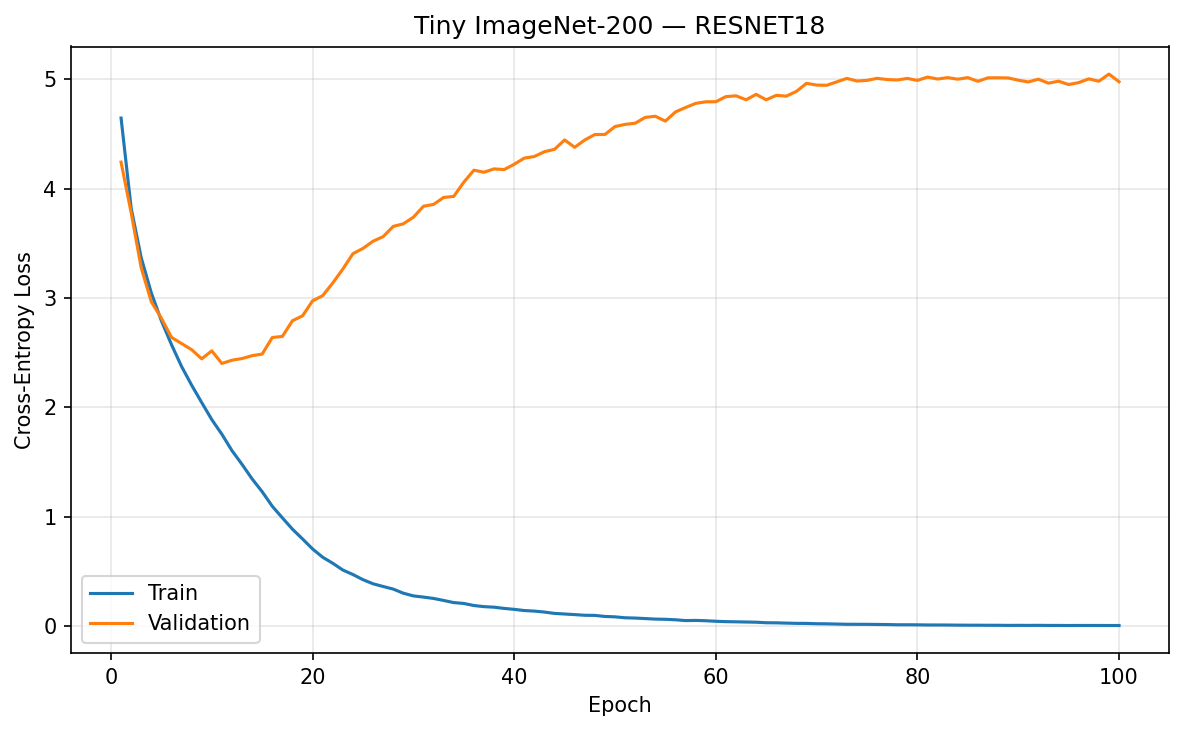
\includegraphics[width=0.48\textwidth]{curves_train_resnet18.png}
  \caption{Train/validation loss curves for ResNet-18 baseline on Tiny ImageNet-200
           (100 epochs, batch 64).}
  \label{fig:curves_resnet18}
\end{figure}

\begin{figure}[H]
  \centering
  \begin{subfigure}[b]{0.48\textwidth}
    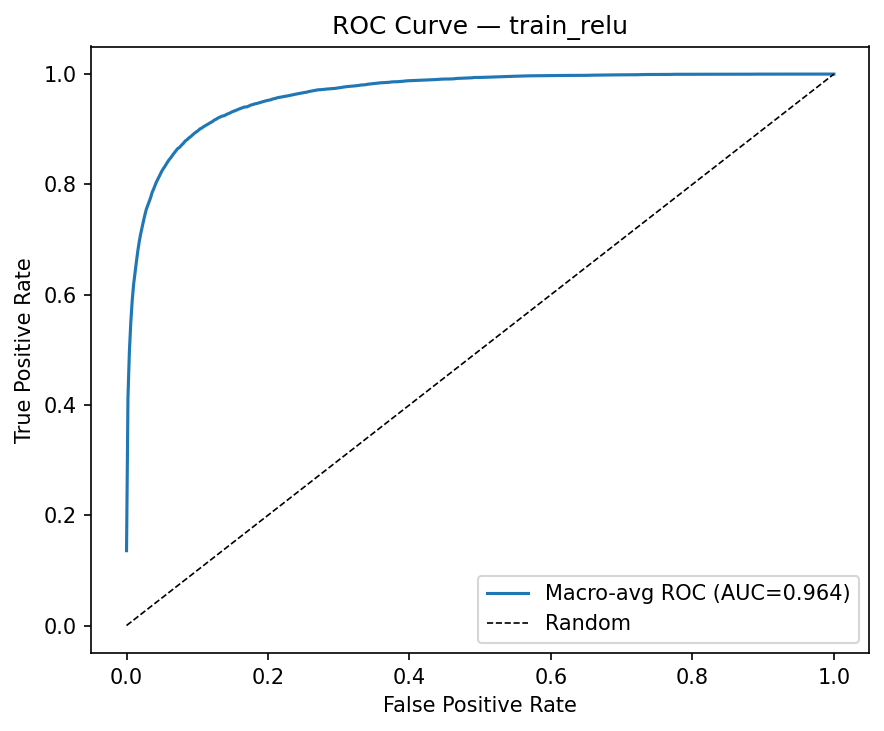
\includegraphics[width=\textwidth]{roc_train_relu.png}
    \caption{ROC --- ReLU (Tiny ImageNet)}
  \end{subfigure}
  \begin{subfigure}[b]{0.48\textwidth}
    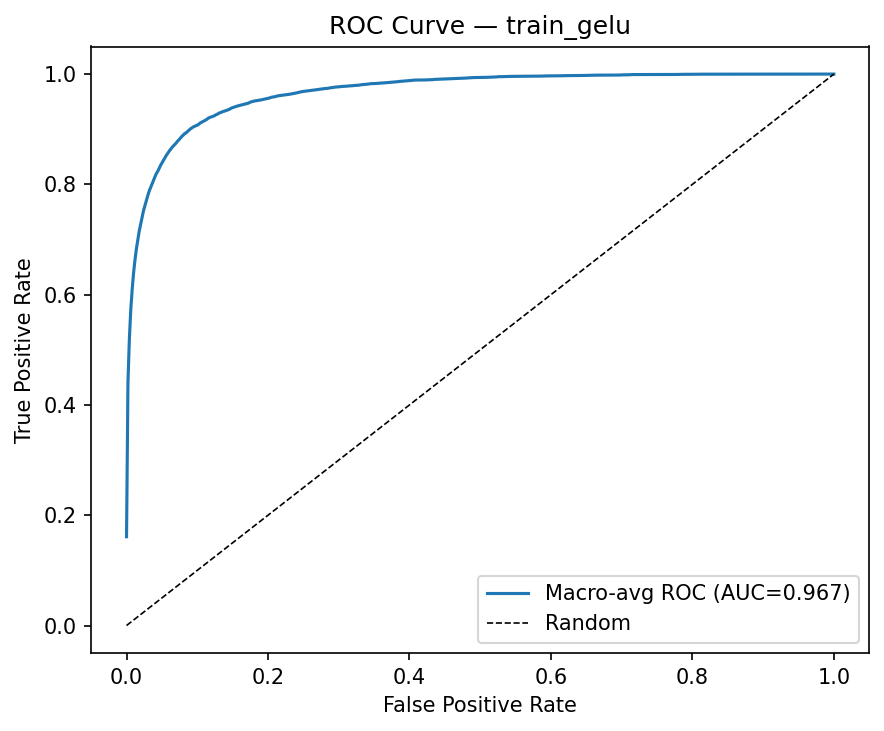
\includegraphics[width=\textwidth]{roc_train_gelu.png}
    \caption{ROC --- GELU (Tiny ImageNet)}
  \end{subfigure}
  \caption{ROC curves for ReLU and GELU on Tiny ImageNet-200.}
  \label{fig:roc_relu_gelu}
\end{figure}

\begin{figure}[H]
  \centering
  \begin{subfigure}[b]{0.48\textwidth}
    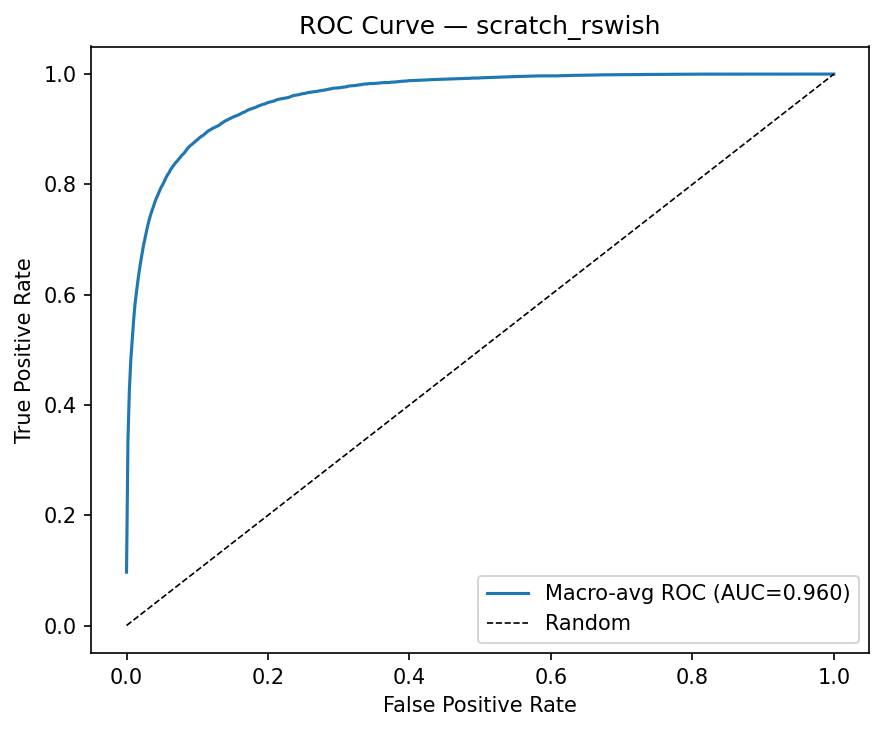
\includegraphics[width=\textwidth]{roc_scratch_rswish.png}
    \caption{ROC --- Scratch (CIFAR-100)}
  \end{subfigure}
  \begin{subfigure}[b]{0.48\textwidth}
    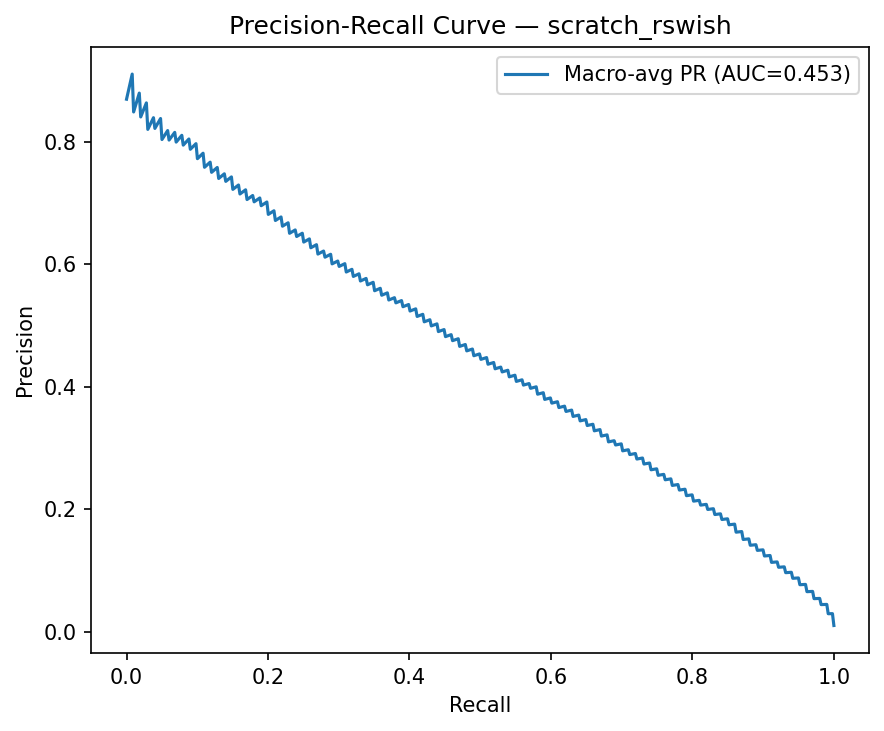
\includegraphics[width=\textwidth]{pr_scratch_rswish.png}
    \caption{PR --- Scratch (CIFAR-100)}
  \end{subfigure}
  \caption{Evaluation of the from-scratch RSwish model on CIFAR-100.}
  \label{fig:eval_scratch}
\end{figure}

\begin{figure}[H]
  \centering
  \begin{subfigure}[b]{0.32\textwidth}
    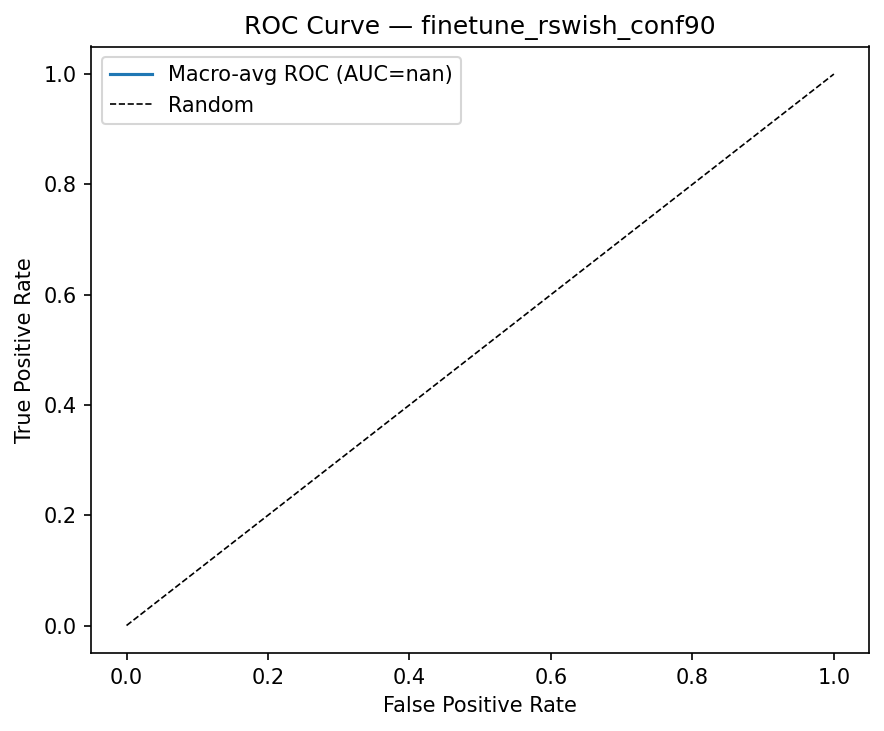
\includegraphics[width=\textwidth]{roc_finetune_rswish_conf90.png}
    \caption{ROC --- Fine-tune ($\geq\!0.9$)}
  \end{subfigure}
  \begin{subfigure}[b]{0.32\textwidth}
    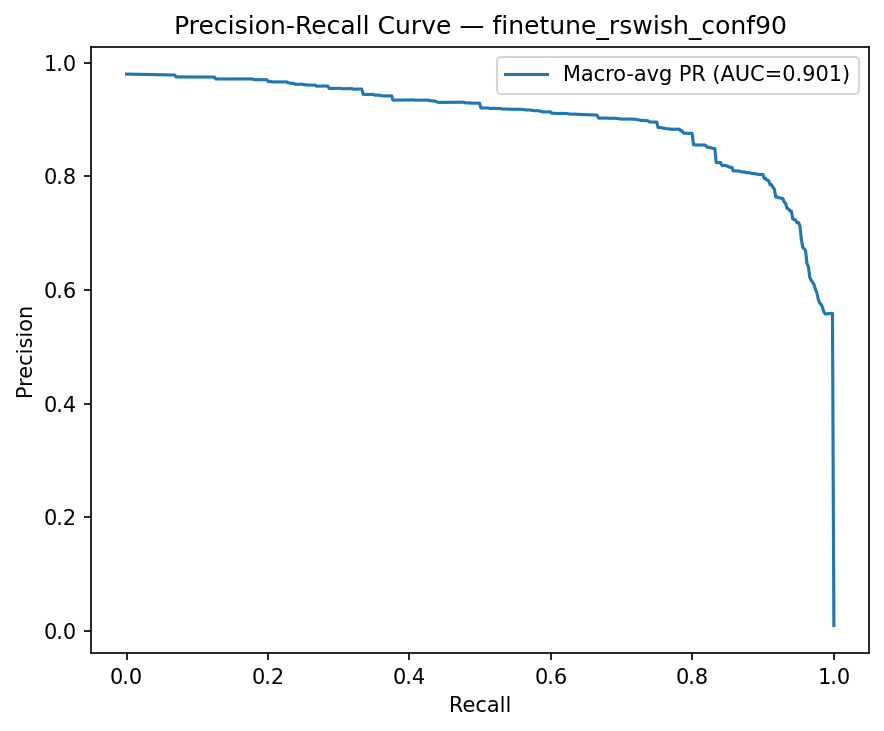
\includegraphics[width=\textwidth]{pr_finetune_rswish_conf90.png}
    \caption{PR --- Fine-tune ($\geq\!0.9$)}
  \end{subfigure}
  \begin{subfigure}[b]{0.32\textwidth}
    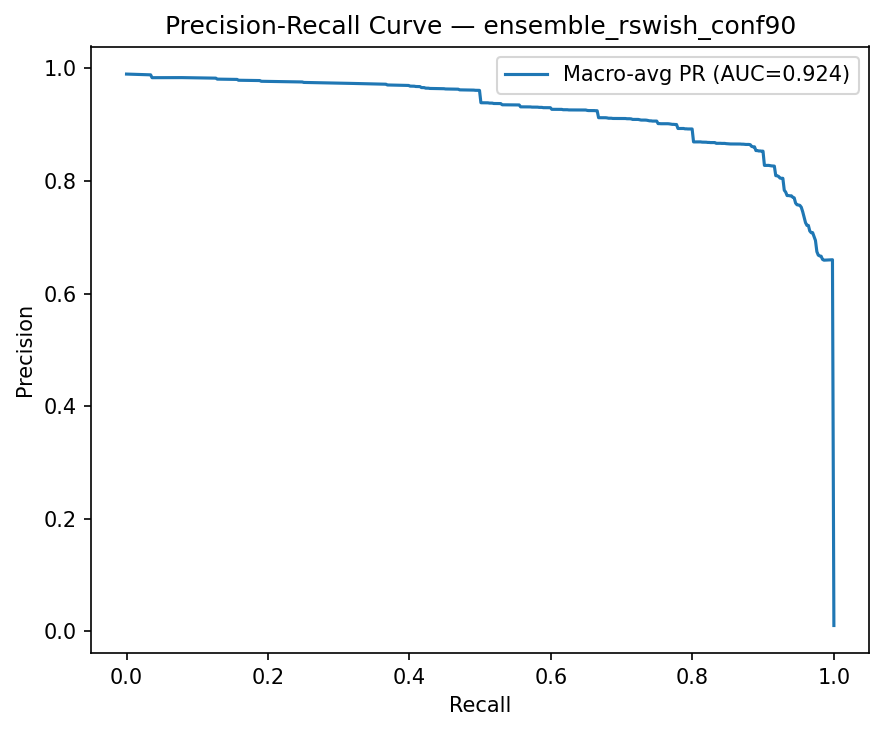
\includegraphics[width=\textwidth]{pr_ensemble_rswish_conf90.png}
    \caption{PR --- Ensemble ($\geq\!0.9$)}
  \end{subfigure}
  \caption{High-confidence evaluation curves on CIFAR-100.}
  \label{fig:conf90_curves}
\end{figure}

\end{document}
